\documentclass[a4paper]{book}

\usepackage{amsmath,longtable,fancyhdr,booktabs,multirow,graphicx,float}
\usepackage{amssymb}
\usepackage{color}
\usepackage[colorlinks,
            linkcolor=black,
            anchorcolor=blue,
            citecolor=green
           ]{hyperref}
\usepackage[top=1in,bottom=1in,left=1.25in,right=1.25in]{geometry}
\usepackage{CJKnumb,titlesec,titletoc}
\usepackage{mnsymbol}
\usepackage{theorem}
\usepackage{algorithmicx}
\usepackage{ulem}

\usepackage[nottoc]{tocbibind}
\def\ci{\perp\!\!\!\perp}
\pagestyle{fancy}
%% define some commands
\newcommand{\normD}{\mathcal{N}}
\newcommand{\mrm}{\mathrm}
\newcommand{\mbf}{\mathbf}
\newcommand{\mcal}{\mathcal}
\newcommand{\ud}{\mathrm{d}}
\newcommand{\e}{\varepsilon}
\newcommand{\up}{\mathrm}
\def\dbar{\mathrm{\mathchar'26\mkern-12mu d}}
\newcommand{\wave}{\scriptsize{\sim}}
\newcommand{\bb}{\mathbb}
\newcommand{\mbb}{\mathbb}
\newcommand{\imp}[1]{\textit{#1}}
\newcommand{\bs}{\boldsymbol}
\newcommand{\mbs}{\boldsymbol}

\DeclareMathOperator*{\argmin}{arg\,min}
\DeclareMathOperator*{\argmax}{arg\,max}
\def\dbar{\mathrm{\mathchar'26\mkern-12mu d}}
\newcommand{\norm}[1]{\left\lVert#1\right\rVert}

\newtheorem{problem}{Problem}
\newtheorem{lemma}{Lemma}
\newtheorem{theorem}{Theorem}
\newtheorem{corollary}{Corollary}
\newtheorem{remark}{Remark}
\newtheorem{observation}{Observation}
\newtheorem{proposition}{Proposition}
\newtheorem{assumption}{Assumption}

\newcommand{\figref}[1]{Fig\onedot~\ref{#1}}
\newcommand{\equref}[1]{Eq\onedot~\eqref{#1}}
\newcommand{\secref}[1]{Sec\onedot~\ref{#1}}
\newcommand{\tabref}[1]{Tab\onedot~\ref{#1}}
\newcommand{\thmref}[1]{Thm\onedot~\ref{#1}}
\newcommand{\prgref}[1]{Program~\ref{#1}}
\newcommand{\clmref}[1]{Claim~\ref{#1}}
\newcommand{\lemref}[1]{Lemma~\ref{#1}}
\newcommand{\propref}[1]{Prop\onedot~\ref{#1}}
\newcommand{\ptyref}[1]{Property\onedot~\ref{#1}}
\newcommand{\yangs}[1]{{\color{cyan}{\bf\sf [YS: #1]}}}
\newcommand{\yang}[1]{{\color{cyan}{\bf\sf [#1]}}}
\newcommand{\Ep}{\mcal{E}}
\newcommand{\Epp}{\widehat{\mcal{E}}_s^+[\mu]}
\newcommand{\Eln}{\widehat{\mcal{E}}_{\lambda,n}[\mu]}
\newcommand{\mup}{\widehat{\mu}_{(X,Y)}^+}
\newcommand{\muln}{\widehat{\mu}_{\lambda,n}}
\newcommand{\Hy}{\mcal{H}_{\mcal{Y}}}
\newcommand{\Hx}{\mcal{H}_{\mcal{X}}}
\newcommand{\HK}{\mcal{H}_{K}}
\newcommand{\HH}{\mcal{H}}
\newcommand{\XX}{\mcal{X}}
\newcommand{\YY}{\mcal{Y}}
\newcommand{\ZZ}{\mcal{Z}}
\newcommand{\BB}{\mcal{B}}
\newcommand{\zz}{\mbf{z}}
\newcommand{\xx}{\mbf{x}}
\newcommand{\yy}{\mbf{y}}
\newcommand{\CC}{\mcal{C}}
\newcommand{\hC}{\widehat{\mcal{C}}}
\def\eg{\emph{e.g}\onedot}
\def\Eg{\emph{E.g}\onedot}
\def\ie{\emph{i.e}\onedot}
\def\Ie{\emph{I.e}\onedot}
\def\cf{\emph{cf}\onedot}
\def\Cf{\emph{Cf}\onedot}
\def\etc{\emph{etc}\onedot}
\def\vs{\emph{vs}\onedot}
\def\wrt{w.r.t\onedot}
\def\dof{d.o.f\onedot}
\def\aka{a.k.a\onedot}
\def\iid{i.i.d\onedot}
\def\etal{\emph{et al}\onedot}

\title{Notes of PRML}
\author{Siyu Wang}
\date{August 2018}

\begin{document}

\maketitle

\chapter{Mathematical Foundations}
\section{Probability Theory}
sum rule: $$p(X) = \sum_Yp(X,Y)$$
product rule: $$p(X,Y) = p(Y|X)p(X)$$
Question: what is the most different thing between bayesian and non-bayesian?
\subsection{probability densities}
continuous variables for $$x = g(y)$$ , $$p_y(y) = p_x(x)|\frac{dx}{dy}| = p_x(g(y))|g'(y)|$$
Bayes' theorem still applies to probability densities or combination of discrete and continuous variables:
$$p(x) = \int p(x, y)\mathrm{d}y$$
$$p(x,y) = p(y|x)p(x)$$
\subsection{Expectations and covariances}
\textit{variance} for one variable $f(x)$: $$\mathrm{var}[f] = E[(f(x)-E[f(x)])^2]$$
\emph{covariance} for two variables $x, y$: $$\mathrm{cov}[x,y]= E_{x,y}[\{x-E[x]\}\{y-E[y]\}]$$
for two vectors of random variables $\textbf{x}$ and $\textbf{y}$, the covariance is a matrix
$$\mathrm{cov}[\textbf{x}, \textbf{y}] =E_{x,y}[\{\textbf{x}-E[\textbf{x} ]\}\{\textbf {y}^T-E[\textbf {y}^T]\}]$$
and for one vector $$\mathrm{cov}[\textbf{x}] = \mathrm{cov}[\textbf {x},\textbf {x}]$$
\subsection{Bayesian probabilities}
essential idea: convert a prior probability into a posterior proboability.
\begin{equation}\label{eq1.1}
  p(\textbf{w},\mathcal{D}) = \frac{p(\mathcal{D}|\textbf {w})p(\textbf {w})}{p(\mathcal{D})}
\end{equation}
note that\newline
$p(\textbf w)$: before observing the data, in the form of a prior probability distribution\newline
$\mathcal{D}$ : observed data $\{t_1,\dots, t_n\}$\newline
$p(\mathcal{D})$ : seen as a normalization constant.\newline
$p(\mathcal{D}|\textbf w)$ : \emph{likelihood function}.  a function of the parameter vector $\textbf w$ , expresses how probable the observed data set is for different settings of the parameter vector $\textbf  w$
key idea can be sumed as:
\begin{equation}\label{eq1.2}
\mathrm{posterior} \propto \mathrm{likelihood} \times \mathrm{prior}
\end{equation}
\textbf{Bayesian and frequentist paradigm}
for frequentist, $\textbf  w$ is considered to be fixed parameter and its vlaue is determined by some form of 'estimator'.\newline
one common frequentist estimator is \emph{maximum likelihood},  maximize likelihood function $p(\mathcal{D}|\textbf w)$, in machine learning, negative lof og the likelihood function is called an \emph{error function}.\newline
\emph{bootstrap} technique.\newline
for Bayesian, there is only a single data set $\mathcal{D}$ and the uncertainty in the parameters is expressed through a probability distribution over $\textbf w$\newline
inclusion of prior knowledge\newline
how to select prior distribution is a problem for Bayesian method.\newline
Reducing the dependence on the prior. \emph{noninformative} priors
\subsection{The Gaussian distribution}
For one variable:
\begin{equation}\label{eq1.3}
  \mathcal{N}(x|\mu,\sigma^2) = \frac{1}{(2\pi\sigma^2)^{1/2}}\exp\{-\frac1{2\sigma^2}(x-\mu)^2\}
\end{equation}
for D-dimensional vector:
\begin{equation}\label{eq1.4}
  \mathcal{N}(\textbf x|\mu, \Sigma) = \frac{1}{(2\pi)^{D/2}}\frac1{|\Sigma|^{1/2}}\exp\{-\frac12(\textbf x-\mu)^T\Sigma^{-1}(\textbf x-\mu)\}
\end{equation}
Problem : observations for N times $\textbf x=(x_1,\dots,x_N)^T$,  we want to get parameters for the Gaussian distribution.
Then the likelihood function$p(\mathcal{D}|\textbf w)$ is just $p(\textbf x|\mu, \sigma^2) = \Pi_{n=1}^{N}\mathcal{N}(x_n|\mu,\sigma^2)$.
so using ML criterion, we will want to maximize $\ln p(\textbf x|\mu,\sigma^2)$ and we can get
$$\mu_{ML} = \frac1N\sum_{n=1}^Nx_n, \mathrm{sample mean}$$,
$$\sigma_{ML}^2 = \frac1N\sum_{n=1}^N(x_n-\mu_{ML})^2, \mathrm{sample variance}$$
but we can infer that:
$$E[\mu_{ML}] = \mu$$
$$E[\sigma_{ML}^2] = (\frac{N-1}N)\sigma^2$$ rather than exactly $\sigma^2$
this can be inferred from inspiration in figure\ref{fig1.1}:
\begin{figure}
  \centering
  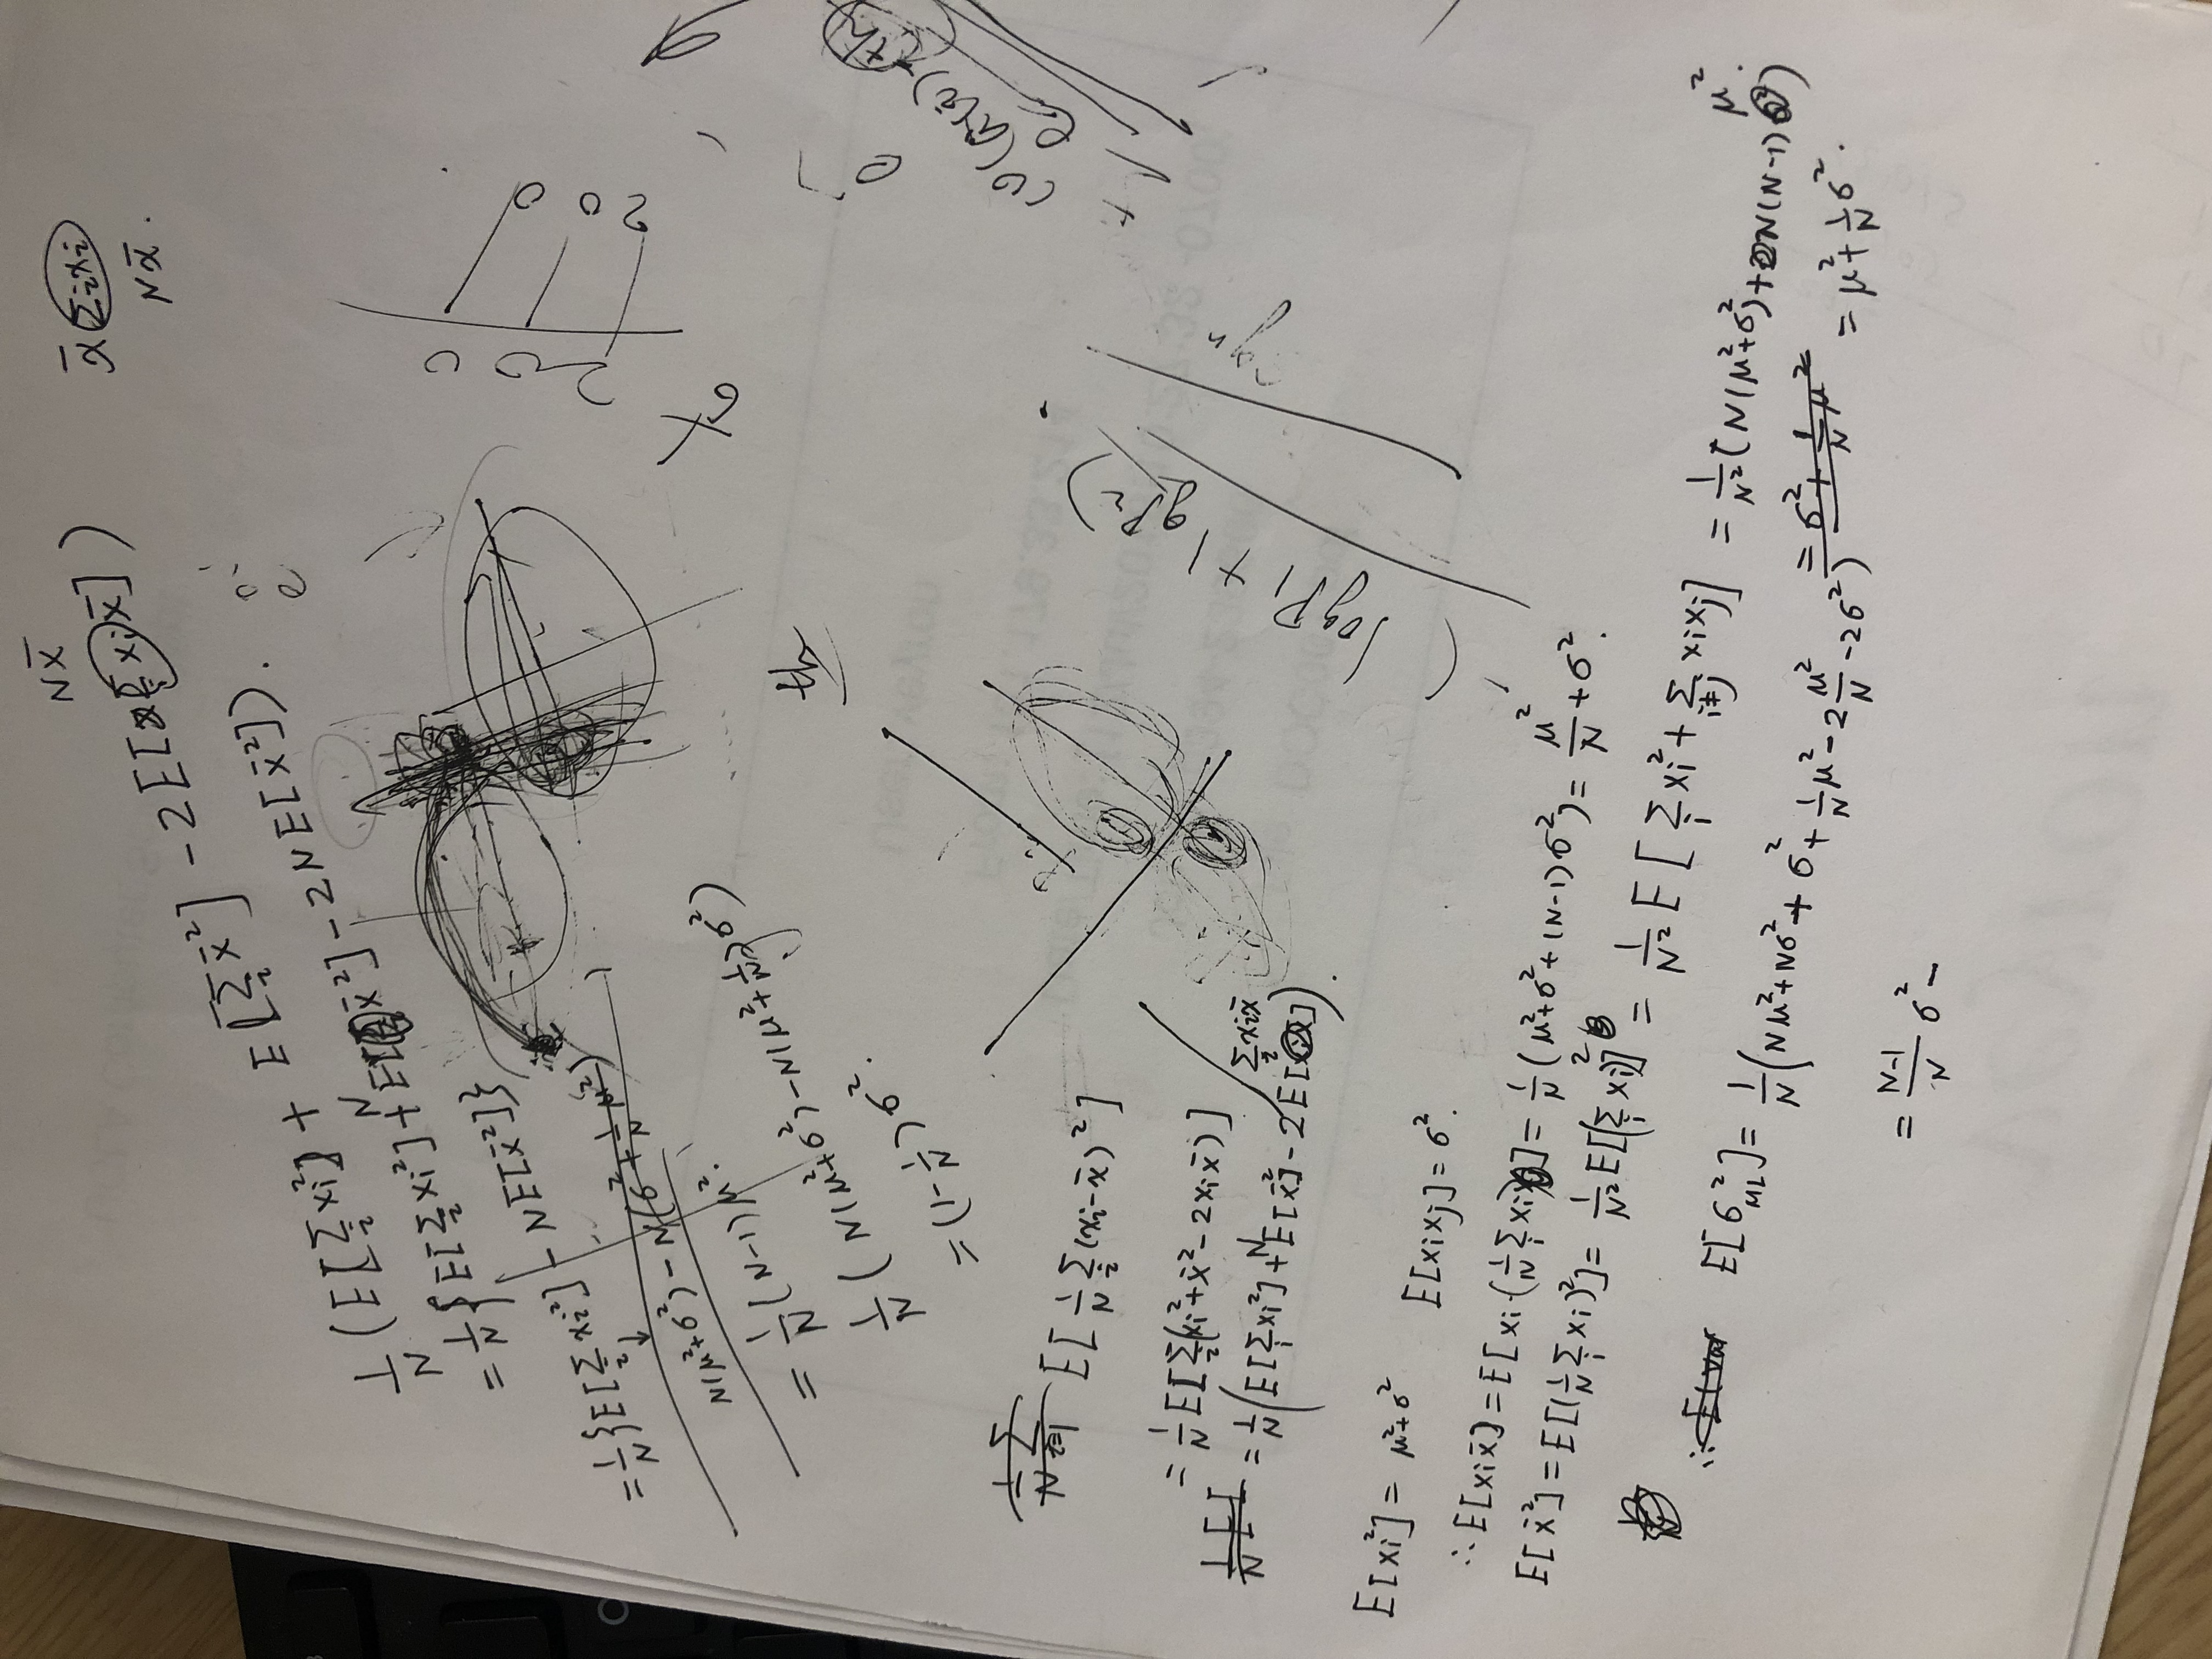
\includegraphics[width=\linewidth]{./imgs/infer1.jpg}
  \caption{Inference}\label{fig1.1}
\end{figure}
but there seems to be more convenient way using chi-sqaure distribution
\subsection{Curve fitting re-visited}
This time, we model curve fitting problem by : given the value of $x$, the corresponding value of $t$ has a Gaussian distribution with a mean equal to the value $y(x,\textbf w)$ (polynomial curve).
\begin{equation}\label{eq1.9}
  p(t|x,\textbf w,\beta) = \mathcal{N}(t|y(x,\textbf w),\beta^{-1})
\end{equation}
\begin{equation}\label{eq1.10}
  p(\textbf t|\textbf x,\mathrm{w},\beta) = \Pi_{n=1}^N\mathcal N(t_n|y(x_n,\mathrm{w}),\beta^{-1})
\end{equation}
and log likelihood function can be derived from above.  and\textbf{
Maximizing likelihood is equivalent to minimizing the sum-of-squares \emph{error function} defined earlier !!!}\newline
if we use Bayesian method and assume prior distribution over \textbf{w}:
\begin{equation}\label{eq1.5}
  p(\mathrm{w}|\alpha) = \mathcal{N}(\mathrm{w}|\textbf{0},\alpha^{-1}\textbf I) )
\end{equation}
$\alpha$ is called \emph{hyperparameters}. Using Bayesian rules to get
\begin{equation}\label{eq1.6}
  p(\mathrm w|\textbf{x}, \textbf t, \alpha,\beta) \propto p(\textbf t|\textbf x,\mathrm w,\beta)p(\mathrm w|\alpha)
\end{equation}
Using \emph{maximizing the posterior distribution, MAP} and we find the maximum of the posterior is given by the minimum of:
\begin{equation}\label{eq1.7}
 \frac{\beta}2\sum_{n=1}^N\{y(x_n,\mathrm{w})-t_n^2+\}\frac{\alpha}2\mathrm{w}^T\mathrm{w}
\end{equation}
so this is similar to regularize sum-od-squares error function with $\lambda=\frac{\alpha}{\beta}$
\subsection{Decision Theory}
\textbf{minimizing the misclassification rate} $p(\mathrm{mistake})$ and $p(\mathrm{correct})$ \newline
\textbf{minimizing the expected loss}\newline
can assign different loss efficient to different error
\begin{equation}\label{eq1.8}
  E[L] = \sum_k\sum_j\int_{\mathcal{R}_j}L_{kj}p(\mathrm{x},\mathcal{C}_k)\mathrm {dx}
\end{equation}
$p(\mathrm{x},\mathcal{C}_k) = p(\mathcal{C}_k|\mathrm{x})p(\mathrm{x})$ to eliminate the common factor $p(\mathrm x)$ \newline
\textbf{ inference and decision}\newline
Three distinct approaches:
\begin{enumerate}
    \item First solve $p(\mrm{x}|\mathcal C_k)$ as well as $p(\mathcal C_k$ for each class individually, then figure out $p(\mathcal C_k|\mrm x) = \frac{p(\mathrm x|\mathcal C_k)p(\mathcal C_k)}{p(\mrm x)}$ and $p(\mrm x)$ can be gotten from $p(\mrm x) = \sum_kp(\mrm x|\mathcal C_k)p(\mathcal C_k)$. This is equivalent to model the joint distribution $p(\mrm x, \mathcal C_k)$
  \item Determine posterior class probabilities $p(\mathcal C_k|\mrm x)$  and then use decision theory.  \emph{discriminative model}.
  \item Find $f(\mathrm x)$ which maps $\mrm{x}$ directly to a class label.
\end{enumerate}
The first approach is too time-consuming and demanding, while the last one is simplest but not so robust as approach.2 because we can see a lot of information from the posterior probabilities:
\begin{itemize}
  \item  minimizing risk,  by adjusting $L_{kj}$ to get different loss function and minimize risk
  \item reject option
  \item \textbf{compensating for class priors} \uline{this is not thought of by myself but very important. sometimes we have to make training set more suitable for learning features, but this operation on training set will lead to a modification on prior probabilities so we must revise this part by divide by the class fraction in the data set and then multiply by the class fraction in the population of which we want to apply this model.}
  \item combining models.
\end{itemize}
\textbf{Loss function for regression}
$$E[L] = \iint L(t,y(\mathrm x))p(\mathrm  x,t)\mathrm {dx}$$
If we define
\begin{equation}\label{eq1.11}
  L(t,y(\mathrm  x)) = \{y(\mathrm  x)-t\}^2
\end{equation}
we can get $y(\mathrm  x) = E_t[t|\mathrm  x]$ to minimize $E[L]$.\newline
Similarly, we also have three approaches using joint probability, posterior probability and a direct regression function $f(\mathrm  x)$\newline
sometimes we define $L$ by \emph{Minkowski} loss as $L_q = |y(\mathrm  x)-t|^q$
\subsection{Information Theory}
Look for a quantity $h(x)$ than is a monotonic function of the probability $p(x)$ and that expresses the information content. and should satisfy
$$h(x,y) = h(x)+h(y)$$.
so we define$$h(x) = -\log_2p(x) (bits)$$  or $$h(x) = -\ln p(x), nats$$
\textbf{ENTROPY}:
\begin{equation}\label{eq1.18}
  H[x] = E[h(x)]= -\sum_xp(x)\log_2p(x)
\end{equation}
relative to \emph{statistical physics}.\newline
To define entropy for continuous variable:\newline
differential entropy: $H[\mathrm x] = -\int p(\mathrm x)\ln p(\mathrm x)$

\textbf{maximizing entropy} by using Lagrange multipliers\newline
\begin{itemize}
  \item for discrete, uniform distribution
  \item  for continuous, Gaussion distribution $H[x] = \frac12[1+\ln (2\pi\sigma^2)]$
\end{itemize}
conditional entropy:
\begin{equation}\label{eq1.12}
H[y|x] = \iint p(y,x)\ln p(y|x) \mathrm dy\mathrm dx
\end{equation}
so  $H[x,y]=H[y|x]+H[x]$.
\subsubsection{Relative entropy and mutual information}
\textbf{KL divergence (relative entropy)}
\begin{equation}\label{eq1.13}
  \mathrm {KL}(p||q) = -\int p(x)\ln q(x)\mathrm dx-(-\int p(x)\ln p(x)\mathrm dx) = -\int p(x)\ln \frac{q(x)}{p(x)}
\end{equation}
this is not symmetrical!\newline
when we use \emph{convex} function and Jensen's unequality,
\begin{equation}\label{eq1.14}
  f(\int xp(x)\mathrm  dx) \leq \int f(x)p(x) \mathrm dx
\end{equation}
also as $f(E[x]) \le E[f(x)]$ we can get
\begin{equation}\label{eq1.14}
  \mathrm  {KL}(p||q) = -\int p(x)\ln\{\frac{q(x)}{p(x)}\}\mathrm  dx \ge -\ln\int q(x)\mathrm  dx = 0
\end{equation}
\uline{BUT I think here, in order to get unequality for KL-divergence , Jensen's unequality should be generalized to $f(E[k(x)])\le E[f(k(x))]$, to be more precise}
the most important thing is , KL divergence can be used as a measure of the dissimilarity of two distributions $p(x)$ and $q(x)$
\subsubsection{to approximate an unknown distribution p(x)}
we have observed a finite set of training points $\mathrm x_n$ for $n=1,2,\dots,N$ drawn from $p(\mathrm  x)$
here we must pay attention that we are not getting points from the distribution curve, we are getting points distributed as $p(\mathrm  x)$ says.
So
\begin{equation}\label{eq1.15}
  \mathrm {KL}(p||q) = -\mathrm  E[\ln\frac{q(\mathrm x)}{p(\mathrm x)}]\simeq\sum_{n=1}^N\{-\ln q(\mathrm  x_n|\theta) +\ln p(\mathrm x_n)\}
\end{equation}
\subsubsection{consider joint distrbiution between two sets of variables x and y}
$p(x,y) = p(x)p(y)$ if x and y is independent.
When they are dependent, we want to use KL divergence between joint distribution and the product of marginals to see how close they are  to independent.
\begin{equation}\label{eq1.16}
  I[x,y] = \mathrm {KL}(p(x,y)||p(x)p(y)) = -\int\int p(x,y)\ln(\frac{p(x)p(y)}{p(x,y)})
\end{equation}
this is \emph{mutual information} between x and y  and
\begin{equation}\label{eq1.17}
I[x,y] = H[x]-H[x|y]
\end{equation}
The mutual information represents the reduction in uncertainty about x as a consequence of the new observation y.
\subsection{Some other distributions}
\subsubsection{Poisson distribution}
\subsubsection{Laplace dsitribution}

\subsection{Conclusion}
The most important thought in this chapter is difference between Bayesian and non Bayesian,, e.g. ML and MAP.  Sometimes ML is equivalent to minimizing error function and MAP can be equivalent to them, too.\newline
The most important thing stepping from non Bayesian to Bayesian, is the inclusion of prior probability and we use $$\mathrm{posterior} \propto \mathrm{likelihood} \times\mathrm{prior}$$
To see this problem from angel of information theory, we can find KL divergence between $p(x,y)$ and $p(x)p(y)$ will be mutual information between x and y. And this represent the reduction in uncertainty about x as a consequence of the new observation y.

\section{Probability Distributions}
In the frequentist treatment , we choose specific values for the parameters by optimizing some criterion, such as the likelihood function. But, in a Bayesian treatment we introduce prior distribution over the parameters and then use Bayes' theorem to compute the corresponding posterior distribution given the observed data.\newline
limitation:  assumes a specific functional form of the distribution.
\subsection{Binary Variables}
\begin{gather}\label{eq1.2.1}
  p(x=1|\mu) = \mu \\
  \mathrm {Bern}(x|\mu) = \mu^x(1-\mu)^{1-x} \\
  \mathrm E[x] = \mu, \mathrm  {var}[x]=\mu(1-\mu)
\end{gather}
data set $\mathcal D={x_1,\dots,x_N}$ of observed values of $x$, independently.\newline
then we can construct the likelihood function
\begin{equation}\label{1.2.2}
p(\mathcal D|\mu) = \Pi_{n=1}^Np(x_n|\mu) = \Pi_{n=1}^N\mu^{x_n}(1-\mu)^{1-x_n}
\end{equation}
log likelihood function $\ln p(\mathcal D|\mu)$\newline
maximize likelihood can lead to $\mu_{ML} = \frac1N\sum_{n=1}^Nx_n$ , and $\sum_{n=1}^Nx_n$ is called \emph{sufficient statistic}\newline
Denote the number of observation of $x = 1 $ within this data set by $m$, then  $\mu_{ML}=\frac mNN$. \newline
\uline{But,we can get extreme result using maximum likelihood criterion!}
\textbf{binomial distribution}
$$\mathrm{Bin}(m|N,\mu) = C_N^m\mu^m(1-\mu)^{N-m} $$
$$\mathrm E[m]=N\mu, \mathrm  {var}[m]=N\mu(1-\mu)$$
\subsubsection{The beta distribution}
we choose an appropriate prior  distribution so that the posterior distribution will have the same functional form as the prior. so \emph{beta distribution} comes.
\begin{gather}\label{1.2.3}
  \mathrm  {Beta}(\mu|a,b) = \frac{\Gamma(a+b)}{\Gamma(a)\Gamma(b)}\mu^{a-1}(1-\mu)^{b-1}
\Gamma(x)=\int_0^\infty u^{x-1}e^{-u}\mathrm du
\end{gather}
The distribution is normalized.
$$\mathrm E[\mu] = \frac a{a+b}, \mathrm {var}[\mu] = \frac{ab}{(a+b)^2(a+b+1)}$$
$a$ and $b$ are \emph{hyperparameters} controlling the distribution of the parameter $\mu$.\newline
so we can get posterior distribution:
$$p(\mu|m,l,a,b) \propto \mu^{m+a-1}(1-\mu)^{l+b-1}$$
and after normalization we get:
$$p(\mu|m,l,a,b) = \frac{\Gamma(m+a+l+b)}{\Gamma(m+a)\Gamma(l+b)} \mu^{m+a-1}(1-\mu)^{l+b-1}$$
The posterior can act as the prior if we subsequently observe additional data.
\emph{sequential approach}:
Sequential methods make use of observations one at a time, or in small batches, and then discard them before the next observations are used.\newline
and
\begin{equation}\label{1.2.4}
  p(x=1|\mathcal D) = \int_0^1p(x=1|\mu)p(\mu|\mathcal D)\mathrm d\mu = \int_0^1\mu p(\mu|\mathcal D)\mathrm d\mu=\mathrm E[\mu|\mathcal D]
\end{equation}
$=\frac{m+a}{m+a+l+b}$\newline
so when $m,l\rightarrow \infty$, it reduce to $\frac{m}{m+l}$\newline
when the number of observations increases, the posterior distribution becomes more sharply peaked, which can be seen from the variance.
\textbf{and this is a general property of Bayesian learning!}\newline
process of inferring can be seen at **page74** in the book.
\subsection{Multinomial Variables}
an extension to binary variables\newline
$\mathrm x = (x_1,\dots,x_K)^T$ one-hot\newline
denote, the probability of $x_k = 1$ by the parameter $\mu_k$ and $\sum_{k=1}^K\mu_k = 1$\newline
so, $p(\mathrm x|\mu) = \Pi_{k=1}^K\mu_k^{x_k}$\newline
data set $\mathcal D$ of $N$ independent observations $\mathrm x_1, \dots, \mathrm x_N$\newline
so likelihood function is:
\begin{equation}\label{1.2.5}
  p(\mathcal D|\mu) = \Pi_{n=1}^N\Pi_{k=1}^K\mu_k^{x_{nk}} = \Pi_{k=1}^K\mu_k^{\sum_nx_{nk}} = \Pi_{k=1}^K\mu_k^{m_k}
\end{equation}
where $m_k = \sum_nx_{nk}$ represents the number of observations of $x_k = 1$, \emph{sufficient statistics} for this distribution\newline
to do ML, maximize $\sum_{k=1}^Km_k\ln \mu_k+\lambda(\sum_{k=1}^K\mu_k-1)$ and we get $\mu_k^{ML} = \frac{m_k}{N}$
\begin{equation}\label{1.2.6}
  \mathrm {Mult}(m_1,\dots,m_K|\mu,N) = \left(\begin{matrix}N\\m_1m_2\dots m_K\end{matrix}\right)\Pi_{k=1}^K\mu_k^{m_k}
\end{equation}
\subsubsection{The Dirichlet distribution}
a family of prior distributions for the parameters $\{\mu_k\}$ of the multinomial distribution.
\begin{equation}\label{1.2.7}
  p(\mu|\alpha) = \frac{\Gamma(\alpha_0)}{\Gamma(\alpha_1)\dots\Gamma(\alpha_K)}\Pi_{k=1}^K\mu_k^{\alpha_k-1}
\end{equation}
 where $\alpha_0 = \sum_{k=1}^K\alpha_k$.
then posterior probability will be $p(\mu|\mathcal D, \alpha) = \mathrm {Dir}(\mu|\alpha+\mathrm m)$
\section{The Gaussian Distribution}
the sum of multiple random variables
\textbf{central limit theorem}
\begin{equation}\label{1.2.8}
  \mathcal N(\mathrm x|\mu, \Sigma) = \frac1{(2\pi)^{D/2}|\Sigma|^{1/2}}\exp\{-\frac12(\mathrm x-\mu)^T\Sigma^{-1}(\mathrm x-\mu)\}
\end{equation}
dependence on $\mathrm x$ is through a quadratic form:
$$\Delta^2 = (\mathrm x-\mu)^T\Sigma^{-1}(\mathrm x-\mu)$$ in the exponent.\newline
We can take $\Sigma$ to be symmetric because ant antisymmetric component would disappear from the exponent.
consider eigenvalues (real number because of $\Sigma$'s reality and symmetry) of $\Sigma$
\begin{equation}\label{1.2.9}
  \Sigma \mathrm u_i= \lambda_i\mathrm u_i, i = 1,2,\dots,D
\end{equation}
$\mathrm u_i^T\mathrm u_j = I_{ij}$

then $\Sigma = \sum_{i=1}^D\lambda_i\mathrm u_i\mathrm u_i^T$ and $\Sigma^{-1} = \sum_{i=1}^D\frac1{\lambda_i}\mathrm u_i\mathrm u_i^T$

and define $y_i=\mathrm u_i^T(\mathrm x-\mu)$,

then $\Sigma^{-1} = \sum_{i=1}^D\frac{y_i^2}{\lambda_i}$

$\mathrm y=\mathrm U(\mathrm x-\mu)$ and $|\mathrm J| = 1$ so $p(\mathrm y) = p(\mathrm x)|\mathrm J| = \Pi_{j=1}^D\frac{1}{(2\pi\lambda_j)^{1/2}}\exp\{-\frac{y_j^2}{2\lambda_j}\}$

\textbf{mean and covariance}
$\mathrm E[\mathrm x] = \mu, \mathrm {cov}[\mathrm x] = \Sigma$

\subsection{Conditional Gaussian distributions}
\begin{equation}\label{1.2.10}
  \mathrm x =(\mathrm x_a^T,\mathrm x_b^T)^T, \mu=(\mu_a^T,\mu_b^T)^T, \Sigma=\left(\begin{matrix}\Sigma_{aa} & \Sigma_{ab}\\\Sigma_{ba} & \Sigma_{bb}\end{matrix} \right)
\end{equation}
we can get
\begin{gather}\label{1.2.11}
  p( \mathrm x_a|\mathrm x_b) = \mathcal N(\mathrm x_a|\mathrm x_b,\mu_{a|b},\Sigma_{a|b}) \\
  \mu_{a|b} = \mu_a+\Sigma_{ab}\Sigma_{bb}^{-1}(\mathrm x_b-\mu_b) \\
  \Sigma_{a|b} = \Sigma_{aa}-\Sigma_{ab}\Sigma_{bb}^{-1}\Sigma_{ba}
\end{gather}
\subsection{Marginal Gaussian distribution}
$p(\mathrm x_a) = \int p(\mathrm x_a,\mathrm x_b)\mathrm d\mathrm x_b$ is
still Gaussian and
$p(\mathrm x_a)= \mathcal N(\mathrm x_a|\mu_a,\Sigma_{aa})$
\subsection{Bayes‘ theorem for Gaussian variable}
\emph{linear Gaussian model}  e.g. Gaussian conditional distribution $p(y|x)$ in which $p(y|x)$ has a mean that is a linear function of $x$, and a covariance which is dependent of $x$. \newline
Our goal: given $p(\mathrm x) = \mathcal {N}(\mathrm x|\mu,\Lambda^{-1})$, $p(\mathrm y|\mathrm x) = \mathcal N(\mathrm y|\mathrm A\mathrm x+\mathrm b,\mathrm L^{-1})$, we want to find  $p(\mathrm y)$ and $p(\mathrm x|\mathrm y)$. \newline
$\mathrm x\in R^M$ and $\mathrm y \in R^D, \mathrm A\in R^{D\times M }$

$$\mathrm z=\left(\begin{matrix}\mathrm x\\\mathrm y\end{matrix}\right)$$
$$\ln p(\mathrm z) =\ln p(\mathrm x)+\ln p(\mathrm y|\mathrm x) $$
and finally $\mathrm z$ has precision matrix as
$$\mathrm R = \left(\begin{matrix}\Lambda+\mathrm A^T\mathrm L\mathrm A&-\mathrm A^T\mathrm L\\-\mathrm L\mathrm A&\mathrm L \end{matrix}\right)$$
and $$\mathrm {cov}[\mathrm z] = \mathrm R^{-1} $$
\begin{figure}
  \centering
  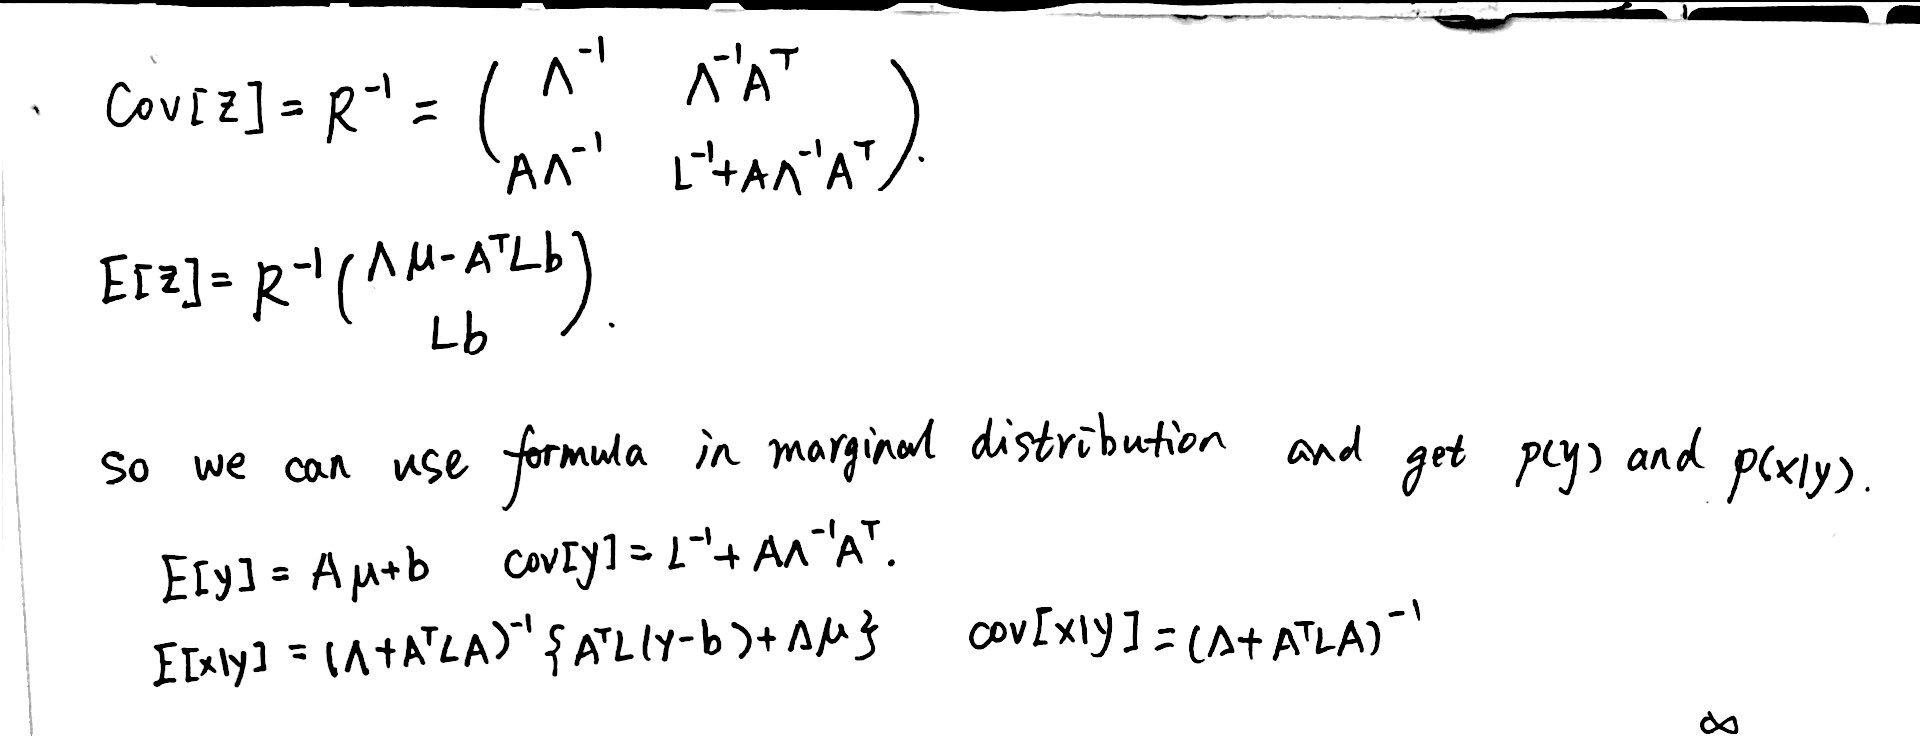
\includegraphics[width=\textwidth]{./imgs/GD1.jpg}
  \label{fig1.1}
\end{figure}
\subsection{Maximum likelihood for the Gaussian }
log likelihood function:
\begin{equation}\label{1.2.12}
  \ln p(\mathrm X|\mu,\Sigma) = -\frac{ND}2\ln(2\pi) - \frac N2\ln|\Sigma|-\frac12\sum_{n=1}^N(\mathrm x_n-\mu)^T\Sigma^{-1}(\mathrm x_n-\mu)
\end{equation}
we should pay attention that the thing on the exponent is a number and
\begin{equation}\label{1.2.13}
  (\mathrm x_n-\mu)^T\Sigma^{-1}(\mathrm x_n-\mu) = \mathrm x_n^T\Sigma^{-1}\mathrm x_n+\mu^T\Sigma^{-1}\mu-2\mathrm x_n^T\Sigma\mu
\end{equation}
\emph{sufficient statistics} for Gaussian distribution $\sum_{n=1}^N\mathrm x_n, \sum_{n=1}^N\mathrm x_n\mathrm x_n^T$ and  $\frac{\partial}{\partial \mu}\ln p(\mathrm X|\mu,\Sigma), \therefore\mu_{ML} = \frac1N\sum_{n=1}^N\mathrm x_n$\newline
$\Sigma_{ML}=\frac1N\sum_{n=1}^N(\mathrm x_n-\mu_{ML})(\mathrm x_n-\mu_{ML})^T $
\newline
and $\mathrm E[\mu_{ML}] =\mu, \mathrm E[\Sigma_{ML}] = \frac{N-1}{N}\Sigma$
\subsection{Sequential estimation}
$\mu_{ML}^{(N)}=\mu_{ML}^{(N-1)}+\frac1N(\mathrm x_N-\mu_{ML}^{(N-1)})$
we will not always be able to derive a sequential algorithm by this route, and so we seek a more general formulation of sequential learning, which  leads us to the \emph{Robbins-Monro} algorithm.
\begin{equation}\label{1.2.14}
  f(\theta) \equiv E[z|\theta] = \int zp(z|\theta)\mathrm dz
\end{equation}
\textbf{regression functions}
goal: to find root for $f(\theta) = 0$\newline
$$\theta^{(N)} = \theta^{(N-1)}+\alpha_{N-1}z(\theta^{(N-1)})$$
$z(\theta^{(N)})$ is an observe value of $z$ when $\theta$ takes the value $\theta^{(N)}$ and $\alpha_N$ should satisfy some conditions.\newline
\textbf{use Robbins Monro algorithm to solve maximizing log likelihood function problem}\newline
We want to get $$\frac{\partial}{\partial\theta}\{\frac{1}{N}\sum_{n=1}^N\ln p(\mathrm x_n|\theta)\} = 0$$
exchanging summation and derivative, taking the limit $N\rightarrow\infty$ and we have
$$\mathrm E_x[\frac{\partial}{\partial \theta}\ln p(x|\theta)]$$
so $$\theta^{(N)} = \theta^{(N-1)}+\alpha_{N-1}\frac{\partial}{\partial\theta^{(N-1)}}\ln p(x_N|\theta^{(N-1)})$$
\subsection{Baysesian inference for the Gaussian}
\begin{itemize}
  \item suppose $\sigma^2$ is known, to get $\mu$
  $$p(X|\mu) = \Pi_{n=1}^Np(x_n|\mu) = \frac1{(2\pi\sigma^2)^{N/2}}\exp\{-\frac1{2\sigma^2}\sum_{n=1}^N(x_n-\mu)^2\}$$
  we choose prior to be Gaussian, too
  $$p(\mu)= \mathcal N(\mu|\mu_0,\sigma_0^2) $$
so $$p(\mu|X) = \mathcal N(\mu|\mu_N,\sigma_N^2)$$
$$\mu_N  = \frac{\sigma^2}{N\sigma_0^2+\sigma^2}\mu_0+\frac{N\sigma_0^2}{N\sigma_0^2+\sigma^2}\mu_{ML}$$
$$\frac1{\sigma_N^2} = \frac1{\sigma_0^2}+\frac N{\sigma^2}$$
when N is infinite large, $\mu_N = \mu_{ML}$, only depend on observations, and $\sigma_N^2$ goes to 0 and the posterior distribution becomes infinitely peaked.\newline
if we take $\sigma_0^2$ to be infinite, so the prior is flat over all real numbers, so prior will be no use.\newline
sequential angle:
$$p(\mu|D)\propto [p(\mu)\Pi_{n=1}^{N-1}p(\mathrm x_n|\mu)]p(\mathrm x_N|\mu)$$
we can view the postrior distribution after N-1 observations as a prior distribution of the Nth observation.
  \item suppose $\mu$ is known, to get $\sigma^2$, see inference in figure\ref{fig1.2}
  \item suppose both are not known. see inference in figure\ref{fig1.3}
\end{itemize}
\begin{figure}
  \centering
  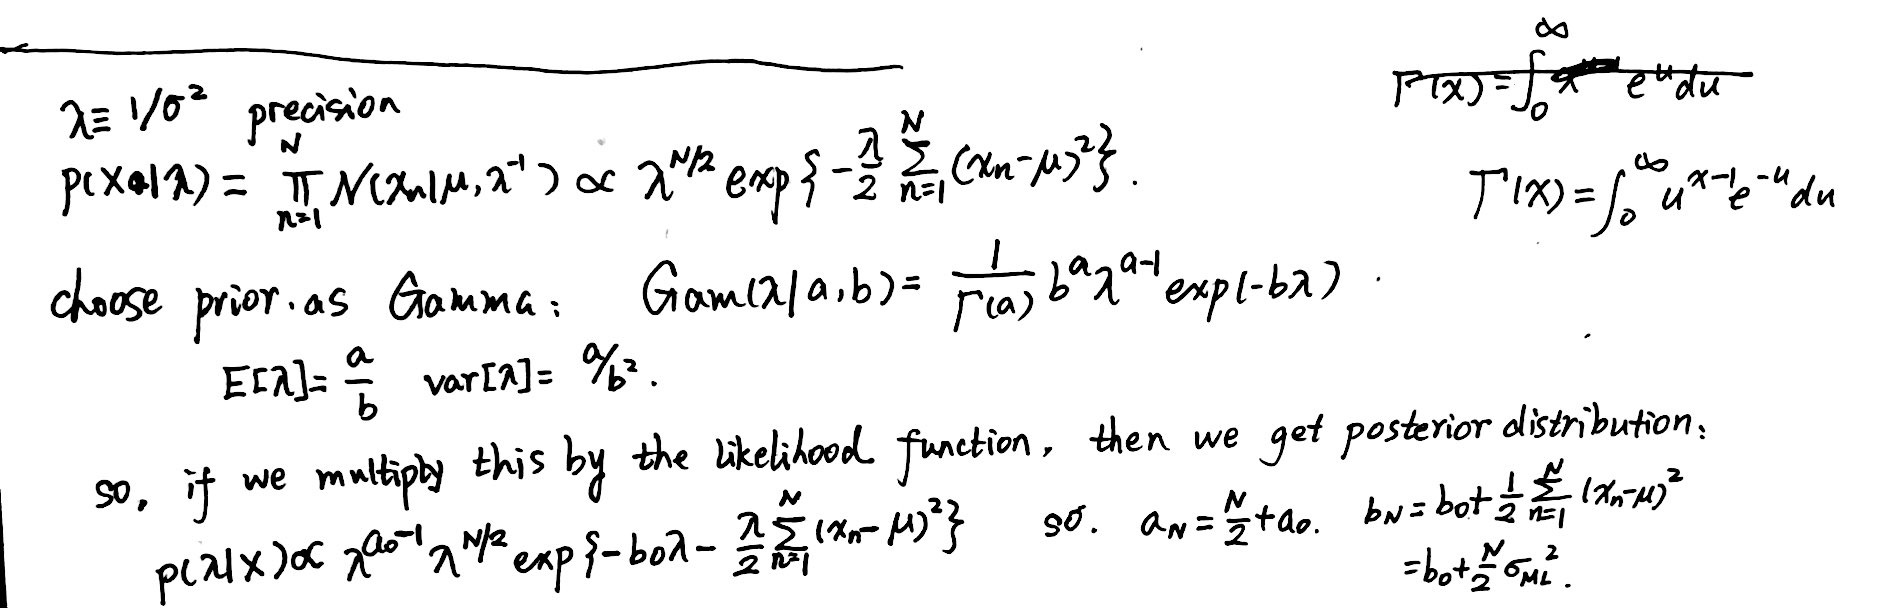
\includegraphics[width=\textwidth]{./imgs/GD2.jpg}
  \label{fig1.2}
\end{figure}
\begin{figure}
  \centering
  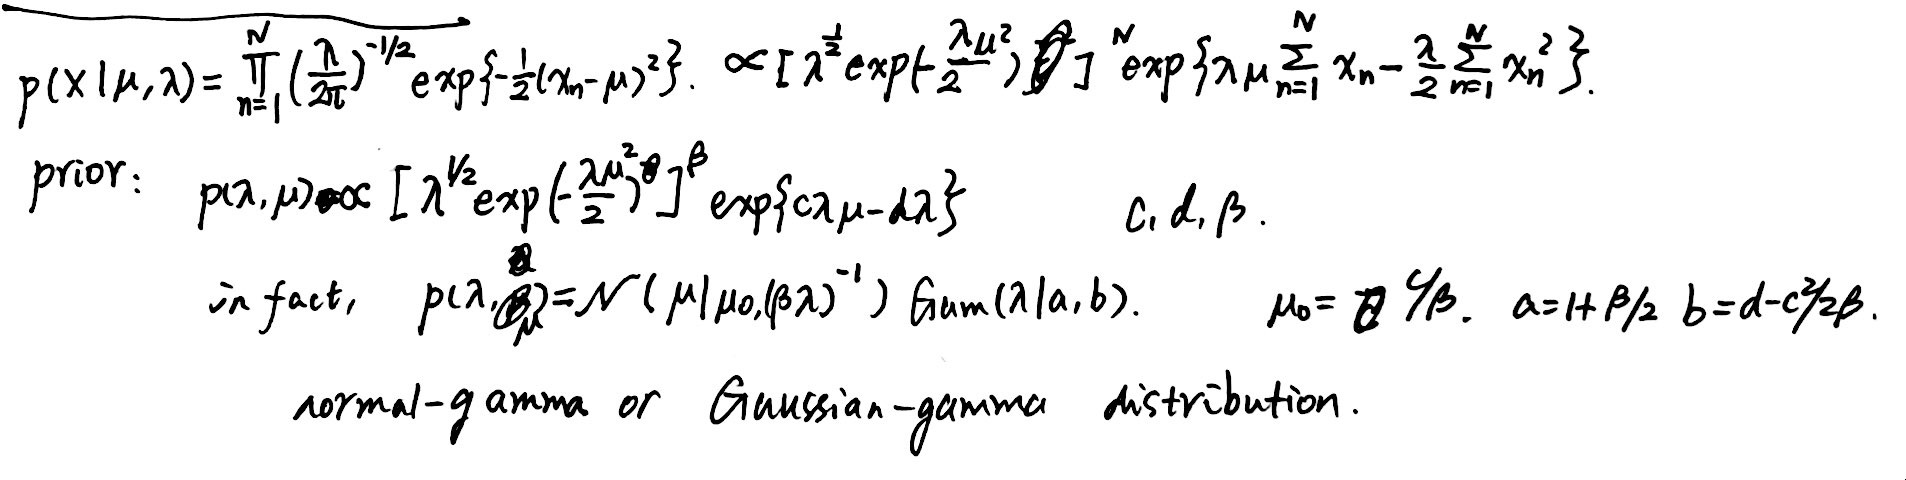
\includegraphics[width=\textwidth]{./imgs/GD3.jpg}
 \label{fig1.3}
\end{figure}
\subsection{Student's t-distribution}
precision $\lambda$    degrees of freedom $\nu$\newline
adding up an infinite number of Gaussian distribution having the same mean but different presicions, we can get Student's t-distribution.
$$\mathrm {St}[x|\mu,\lambda,\nu] = \frac{\Gamma(\nu/2+1/2)}{\Gamma(\nu/2)}{(\frac{\lambda}{\pi\nu})^{1/2}}[1+\frac{\lambda(x-\mu)^2}{\nu}]^{-\nu/2-1/2}$$
Data set: $(x_1,x_2,...,x_N)^T, (t_x,t_2,...,t_N)^T$.\newline
there is noise on the observation !
fit the data using a polynomial function:
\begin{equation}\label{2.1}
y(x, \textbf{w}) = w_0+w_1x+w_2x^2+\dots+w_Mx^M=\sum_{j=0}^Mw_jx^j
\end{equation}
this is a \textbf{linear} function of coefficients $\bf{w}$  !! so this is linear.
goal is to minimize:
\begin{equation}\label{2.2}
E(\textbf{w}) = \frac12\sum_{n=1}^N\{y(x_n,\textbf{w})-t_n\}^2
\end{equation}
\textit{this is a quadratic function of w so its derivatives with respect to coefficients will be linear so the minimization of the error function has a unique solution.}
\subsection{Mixtures of Gaussians}
$$p(\mathrm x) = \sum_{k=1}^K\pi_k\mathcal N(\mathrm x|\mu_k, \Sigma_k)$$
$$\sum_{k=1}^K \pi_k= 1$$

likelihood function:
$$\ln p(\mathrm X|\pi,\Sigma,\mu) = \sum_{n=1}^N\ln\{\sum_{k=1}^K\pi_k\mathcal N(\mathrm x_n|\mu_k,\Sigma_k)\}$$
this is more complex than a single Guassian because the presence of summation over $k$ inside the logarithm.  we can use EM algorithm later .

\section{The Exponential Family}
definition:
\begin{equation}\label{eq1.4.1}
  p(\mathrm x|\eta) = h(\mathrm x)g(\eta)\exp(\eta^T\mathrm u(\mathrm x))
\end{equation}
$g(\eta)$ is to normalize the function $g(\eta) \int h(\mathrm x)\exp(\eta^T\mathrm u(\mathrm x))\mathrm {dx} = 1$\newline
\textbf{Bernoulli}
\begin{equation}\label{1.4.2}
  p(x|\mu) =  \mu^x(1-\mu)^{1-x} = \exp\{x\ln\mu+(1-x)\ln(1-\mu)\} = (1-\mu)\exp\{\ln(\frac{\mu}{1-\mu})x\}
\end{equation}
so we define $\eta = \ln\frac{\mu}{1-\mu}$ so $\mu = \sigma(\eta) \frac{1}{1+\exp(-\eta)}$ \emph{logistic sigmoid function}
$u(x) = x, h(x) = 1, g(\eta) = \sigma(-\eta)$
\subsection{Maximum likelihood and sufficient statistics}
\begin{equation}\label{1.4.3}
  \mathrm  \nabla g(\eta) \int h(\mathrm  x)\exp\{\eta^T\mathrm  u(\mathrm  x)\}\mathrm  {dx} +g(\eta)\int h(\mathrm  x)\exp\{\eta^T\mathrm u(\mathrm x)\} \mathrm u(\mathrm  x) \mathrm {dx} = 0
\end{equation}
so $-\nabla \ln g(\eta) = \mathrm E[\mathrm  u(\mathrm  x)] $\newline
so consider
$$p(X|\eta)  = (\Pi_{n=1}^Nh(\mathrm  x_n))g(\eta)^N\exp\{\eta^T\sum_{n=1}^N\mathrm  u(\mathrm  x_n) \}$$
set the gradient to zero and we get
\begin{equation}\label{1.4.4}
  -\nabla \ln g(\eta_{ML} ) = \frac1N\sum_{n=1}^N\mathrm  u(\mathrm  x_n)
\end{equation}
$\sum_n\mathrm  u(\mathrm  x_n)$ is the sufficient statistics of the distribution.
\subsection{Conjugate priors}
for any member of the exponential family, there exist a conjugate  prior:
$$p(\eta|\chi, \nu) = f(\chi,\nu)g(\eta)^\nu\exp\{\nu\eta^T\chi\}$$
so the posterior distribution can be figured out as the same form:
$$p(\eta|X,\chi,\nu) \propto g(\eta)^{\nu+N}\exp\{\eta^T(\sum_{n=1}^N\mathrm  u(\mathrm  x_n)+\nu\chi)\}$$
\subsection{Noninformative priors}
to have little influence on the posterior distribution, we seek a form of prior distribution called \emph{a noninformative prior}.






\section{Laplace Approximation}
In this chapter, we mainly want to solve the problem that when the posterior distribution is no longer Gaussian, how can we integrate exactly over the parameter vector.\newline
So Laplace approximation can help us to transform a non-Gaussian distribution  into a Gaussian distribution.
\section{Hessian Matrix}
\section{FOR NEW}

\chapter{Models}
\section{Polynomial Curve Fitting}
$\textbf{x} = (x_1,x_2,\dots, x_N)^T $ and $\textbf{t} =(t_1,t_2, \dots, t_N)^T$
There is noise on the observation !\newline
Fit the data using a polynomial function:
$$y(x, \textbf{w}) = w_0+w_1x+w_2x^2+\dots+w_Mx^M=\sum_{j=0}^Mw_jx^j$$
This is a \textbf{linear} function of coefficients \textbf{w}  !! So this is linear.\newline
Goal is to minimize:
$$E(\textbf{w}) = \frac12\sum_{n=1}^N\{y(x_n,\textbf{w})-t_n\}^2$$
\emph{This is a quadratic function of w so its derivatives with respect to coefficients will be linear so the minimization of the error function has a unique solution.}
\subsection{the influence of order M}
define error by root-mean-square:
\begin{equation}\label{2.3}
E_{RMS} = \sqrt{2E(\textbf{w}^*)/N}:
\end{equation}
too small: not enough.\newline
too large: \textbf{overfitting} and large coefficients, very sensitive to \textbf{noise}! low training error while large testing error.
\subsection{the influence of size of training set}
increasing the size of the data set reduces the over-fitting priblem.\newline
\textunderscore{\emph{comment}: this is obvious because the when the size of data set gets larger, the order will become smaller relatively. the requirement for over-fitting is larger order. but when we choose the complexity of our model, we can not depend on the size of data set, we must choose more robust model for \textbf{specific problem}.}
\subsection{modifying error function to solve overfitting}
\begin{equation}\label{2.4}
\tilde{E}(\textbf{w}) = \frac12\sum_{n=1}^M\{y(x_n,\textbf{w})-t_n\}^2+\frac{\lambda}{2}||\textbf{w}||^2
\end{equation}
\emph{regularizier} $$||\textbf{w}||^2 = w_0^2+\dots+w_M^2$$
\emph{somtimes $w_0$ is omitted to exclude the effect of origin for the tarfet variable !!}
in nerual networks, this approach is known as \emph{weight decay}
To optimize $M$ and $\lambda$, we sometimes divide dataset into \emph{training} and \emph{validation} but this is a waste, so we need more sophisticated approaches.






\section{Linear Models for Regression}
\subsection{Linear Basis Function Models}
input $\mathrm x\in R^D$
\begin{equation}\label{eq2.2.1}
  y(\mathrm x,\mathrm w) = w_0+w_1x_1+\dots +w_Dx_D
\end{equation}
extend to nonlinear function of $\mathrm x$ and $y(\mathrm x,\mathrm w) =\mathrm w^T\phi(\mathrm x)$, there are M basis functions $\phi_j(\mathrm x), j=1,2\dots,M$ and $\phi_0(\mathrm x) = 1$\newline
so $\mathrm w\in R^M$
\textbf{normal basis functions}
\begin{itemize}
  \item polynomial $\phi_j(x) = x$
  \item Gaussian $\phi_j(x) = \exp\{-\frac{(x-\mu_j)^2}{2s^2}\}$
  \item sigmoidal $\phi_j(x) = \sigma(\frac{x-\mu_j}{s}) , \sigma(a) = \frac1{1+\exp(-a)}$ sigmoid is equivalent to 'tanh' function.
\end{itemize}
\subsubsection{Maximum likelihood and least squares}
$$t = y(\mathrm x,\mathrm w)+\epsilon, \epsilon\sim\mathcal N(0,\beta^{-1}), \beta = \sigma^{-2}$$
so $$p(t|\mathrm x,\mathrm w,\beta) = \mathcal N(t|y(\mathrm x,\mathrm w),\beta^{-1})=\frac{1}{\sqrt{2\pi/\beta}}\exp\{-\frac{\beta(t-y(\mathrm x,\mathrm w))^2}{2}\}$$
$$\mathrm E[t|\mathrm x] =\int t p(t|\mathrm x)\mathrm dt=y(\mathrm x,\mathrm w)$$
for $N$ observations,
$$p(\mathrm t|\mathrm X,\mathrm w,\beta) = \Pi_{n=1}^N\mathcal N(t_n|\mathrm w^T\phi(\mathrm x_n), \beta^{-1})$$
we can ignore $\mathrm X$ in he condition and get likelihood function:
$$\ln p(\mathrm t|\mathrm w,\beta) = \sum_{n=1}^N\ln \mathcal N(t_n|\mathrm w^T\phi(\mathrm x_n),\beta^{-1}) = \frac N2\ln\beta-\frac N2\ln(2\pi)-\beta E_D(\mathrm w)$$
in which, $$E_D(\mathrm w) = \frac12\sum_{n=1}^N\{t_n-\mathrm w^T\phi(\mathrm x_n)\}^2$$
use maximum likelihood to determine $\mathrm w$ and $\beta$, we get
\begin{equation}\label{3.2.2}
  \nabla \ln p(\mathrm t|\mathrm w,\beta) = \sum_{n=1}^N\{t_n-\mathrm w^T\phi(\mathrm x_n)\}\phi(\mathrm x_n)^T = 0
\end{equation}
and we obtain
$$\mathrm w_{ML} = (\Phi^T\Phi)^{-1}\Phi^T\mathrm t$$
here $\Phi$ is an $N\times M$ matrix called the \emph{design matrix}, and $\Phi_{nj} = \phi_j(\mathrm x_n)$
\uline{so each row of $\Phi$ is dependent on the same observation and each column is dependent on the same basis function.} \newline
$\Phi^{\dagger} = (\Phi^T\Phi)^{-1}\Phi^T$ is known as the *Moore-Penrose pseudo-inverse* of the matrix.\newline
For $w_0$, we can see $w_0=\bar t-\sum_{j=1}^{M-1}w_j\bar \phi_j$, where $\bar t=\frac1N\sum_{n=1}^Nt_n, \bar{\phi_j}=\frac1N\sum_{n=1}^N\phi_j(\mathrm x_n)$. So the bias $w_0$ compensates for the different between the averages of the target values and the weighted sum of the averages of the basis function values. Also we can get$1/\beta_{ML}=\frac1N\sum_{n=1}^N\{t_n-\mathrm w_{ML}^T\phi(\mathrm x_n)\}^2$
\subsubsection{Geometry of least squares}
$\mathrm t=(t_1,\dots,t_N)^T$ is a vector in N-dimensional space. Define $\mathrm y$ to be an N-dimensional vector whose $n^{th}$ element is given by $y(\mathrm x_n,\mathrm w)$,  so $\mathrm y$ is an arbitrary linear combination of the vectors $\varphi_j$, it can live anywhere in the M-dimensional subspace.\newline
Thus the least-squares solution for $\mathrm  w $ corresponds to that choice of $\mathrm y$ that lies in subspace $S$ and that is closest to t. so we choose the orthogonal projection of $\mathrm t$  onto the subspace.\newline
some problems: singularity of $\Phi^T\Phi$
\subsubsection{Sequential learning}
SGD (\emph{stochastic gradient descent}, aka, \emph{sequential gradient descent})\newline
$$\mathrm w^{(\tau+1)}=\mathrm w^{(\tau)}-\eta\nabla E_n$$
So for the case of the sum-of-squares erroe function, this gives
$$\mathrm w^{\tau+1}=\mathrm w^{(\tau)}+\eta(t_n-\mathrm w^{(\tau)^T}\phi_n)\phi_n$$ where $\phi_n=\phi(\mathrm x_n)=(\phi_1(\mathrm x_n), \dots, \phi_M(\mathrm x_n))^T$
\emph{least-mean-squares} algorithm (\emph{LMS})
\subsubsection{Regularized least squares}
Total error function to be minimized takes the from :
$E_D(\mathrm w) +\lambda E_W(\mathrm w)$ Usually, $E_W(\mathrm w) = \frac12\mathrm w^T\mathrm w$ And we can obtain $\mathrm w=(\lambda\mathrm I+\Phi^T\Phi)^{-1}\Phi^T\mathrm t$ by setting the gradient of total error function with respect to $\mathrm w$ to zero.
\subsubsection{Multiple outputs}
$\mathrm t\in R^K, K>1$ is the outputs.\newline
$\mathrm y(\mathrm x,\mathrm W) =W^T\phi(\mathrm x)$
$W\in R^{M\times K }, \phi(\mathrm x)$ is a $M$-dimensional column vector with elements $\phi_j(\mathrm x)$ with $\phi_0(\mathrm x) = 1$.\newline
$M$: the number of basis functions $\phi_1(\mathrm x), \dots, \phi_M(\mathrm x)$\newline
$K$: outputs are in K-dimensional space.
$$p(\mathrm t|\mathrm x,\mathrm W,\beta) = \mathcal N(\mathrm t|\mathrm W^T\phi(\mathrm x),\beta^{-1}\mathrm I)$$
If we have $N$ observations, $\mathrm t_1,\dots,\mathrm t_N$, into one matrix $\mathrm T\in R^{N\times K}$, combine $\mathrm x_1,\dots,\mathrm x_N$  into one  matrix $\mathrm X\in R^{N\times D}$
\begin{equation}\label{eq2.2.3}
  \ln p(\mathrm T|\mathrm X,\mathrm W,\beta) = \sum_{n=1}^N\ln\mathcal N(\mathrm t_n|\mathrm W^T\phi(\mathrm x_n), \beta^{-1}\mathrm I) = \frac{NK}{2}\ln(\frac{\beta}{2\pi})-\frac{\beta}{2}\sum_{n=1}^N||\mathrm t_n-\mathrm W^T\phi(\mathrm x_n)||^2
\end{equation}
and we can get $\mathrm W_{ML} = (\Phi^T\Phi)^{-1}\Phi^T\mathrm T$, $\mathrm w_k = (\Phi^T\Phi)^{-1}\Phi^T\mathrm t_k$

\subsection{The Bias-Variance Decomposition}
don't quite understand:\newline
\uline{distinguishing between the squared loss function arising from decision theory and the sum-of-squares error function that arose in the maximum likelihood estimation of model parameter.}
denote $h(\mathrm x) = \mathrm E[t|\mathrm x] = \int tp(t|\mathrm x)\mathrm dt$. If we have unlimited data set $\mathcal D$, how can be get $h(\mathrm x)$?

\subsection{ Bayesian Linear Regression}
Because effective model complexity, governed by the number of basis functions, needs to be controlled according to the size of the data set, the issue of deciding the appropriate model complexity for the particular problem which cannot be decided simply maximizing the likelihood function still exists. So we turn to Bayesian treatment of linear regression and we can avoid the over-fitting problem and also lead to automatic methods of determining model complexity using the training data alone.
\subsubsection{Parameter distribution}
we assume that precision parameter $\beta$ is known and the prior  probability distribution is as the form:
\begin{equation}\label{eq2.2.4}
  p(\mathrm w) =\mathcal N(\mathrm w|\mathrm m_0,\mathrm S_0)
\end{equation}
so the posterior probability will be Gaussian, too
\begin{equation}\label{eq2.2.5}
  p(\mathrm w|\mathrm t) = \mathcal N(\mathrm w|\mathrm m_N,\mathrm S_N)
\end{equation}
where $\mathrm m_N=\mathrm S_N(\mathrm S_0^{-1}\mathrm m_0+\beta \Phi^T\mathrm t)$ and $\mathrm S_N^{-1}=\mathrm S_0^{-1}+\beta\Phi^T\Phi$\newline
To simplify the model we assume $\mathrm S_0 = \alpha^{-1}\mathrm I$ and $ \mathrm m_0=\mathrm 0$. Then, maximization of this posterior distribution with respect to $\mathrm w$ is therefore equivalent to minimization of the sum-of-square error function with the addition of a quadratic regularization term.
\subsubsection{Predictive distribution }
In practice, we only want to predict t for new values of $\mathrm x$ rather than $\mathrm w$. So we evaluate the \emph{predictive distribution} defined by
\begin{equation}\label{eq2.2.6}
  p(t|\mathrm t,\alpha,\beta) = \int p(t|\mathrm w,\beta)p(\mathrm w|\mathrm t,\alpha,\beta)\mathrm {dw}
\end{equation}
\subsubsection{Equivalent kernel }
We see that the predictive mean can be written in the form
$$y(\mathrm x,\mathrm m_N) =\mathrm m_N^T\phi(\mathrm x)=\beta\phi(\mathrm x)^T\mathrm S_N\Phi^T\mathrm t=\sum_{n=1}^N\beta\phi(\mathrm x)^T\mathrm S_N\phi(\mathrm x_n)t_n$$
we can define kernel
$k(\mathrm x,\mathrm x') = \beta\phi(\mathrm x)^T\mathrm S_N\phi(\mathrm x')$ is known as the *smoother matrix* or *equivalent kernel*. make predictions by taking linear combinations of the training set target values.
\subsection{Bayesian Model Comparison}
Consider the problem of model selection from a Bayesian perspective by simply involving the use of probabilities to represent uncertainty in the choice of model.\newline
Given a training seet $\mathcal D$ we wish to evaluate the posterior distribution $p(\mathcal M_i|\mathcal D) \propto p(\mathcal M_i)p(\mathcal D|\mathcal M_i)$\newline
the prior shows our preference for different models.\newline
If we choose $p(\mathcal M_i)$ to be identical, then the interesting term is the model evidence $p(\mathcal D|\mathcal M_i)$.\newline
the model evidence is sometimes called \emph{marginal likelihood.}
We can conclude that the Bayesian framework avoids the problem of over-fitting  and allows models to be compared on the basis of the training data alone. However, we still needs to make assumptions about the form of the model.
\subsection{The Evidence Approximation}
\subsection{Limitations of Fixed Basis Functions}
basis function $\phi_j(\mathrm x)$ are fixed before the training data set is observed.\newline

curse of dimensionality




\section{Linear Models for Classification}
This chapter aims to solve classification tasks linear models.\newline
Three approaches:
\begin{itemize}
  \item discriminant function, directly assigns each vector $\mathrm x$ to a specific class.
  \item models conditional probability distribution $p(\mathcal C_k|\mathrm x)$ in an inference stage and then subsequently uses this distribution to make optimal decisions:
      \begin{itemize}
        \item directly model the conditional probability
        \item generative approach. model the class-conditional densities given by $p(\mathrm x|\mathcal C_k)$, together with the prior probabilities $p(\mathcal C_k)$
      \end{itemize}
\end{itemize}
No longer linear in the parameters due to the presence of the nonlinear activation function.
\subsection{Discriminant Functions}
$$y(\mathrm x) = \mathrm w^T\mathrm x+w_0$$
and the decision surface is given by $\frac{\mathrm w^T\mathrm x}{||\mathrm w||} = -\frac{w_0}{||\mathrm w||}$
for multiple classes,  it's kind of difficult to reduce to 2-class. a single $K$-class discriminant comprising $K$ linear functions of the form:
$y_k(\mathrm x) = \mathrm w_k^T\mathrm x+w_{k0}$ and then assigning a point $\mathrm x$ to class $\mathcal C_k$ if $y_k(\mathrm x)$ is the largest.\newline
approaches to learning the discriminant functions:
\begin{itemize}
  \item least squares for classification
  \item fisher's linear discriminant
  \item perceptron algorithm
\end{itemize}
\subsection{Probabilistic Generative Models}
logistic sigmoid function and softmax function\newline
assume the class-conditional densities are Gaussian. assume the same covariance matrix.
\begin{equation}\label{2.3.1}
  p(\mathrm x|\mathcal C_k) = \frac{1}{(2\pi)^{D/2}}\frac{1}{|\Sigma|^{1/2}}\exp\{-\frac12(\mathrm x-\mu_k)^T\Sigma^{-1}(\mathrm x-\mu_k)\}
\end{equation}
for two-class case $p(\mathcal C_1|\mathrm x) = \sigma(\mathrm w^T\mathrm x+w_0)$\newline
where $\mathrm w = \Sigma^{-1}(\mu_1-\mu_2)$, $w_0 = -\frac12\mu_1^T\Sigma^{-1}\mu_1+\frac12\mu_2^T\Sigma^{-1}\mu_2+\ln\frac{p(\mathcal C_1)}{p(\mathcal C_2)}$\newline
for K classes we have  $a_k(\mathrm x) \mathrm w_k^T\mathrm x+w_{k0}$ where $ \mathrm w_k = \Sigma^{-1}\mu_k, w_{k0} = -\frac12\mu_k^T\Sigma^{-1}\mu_k+\ln p(\mathcal C_k)$
\newline
Then, we can determine the vlaues of the parameters, together with the prior class probabilities $p(\mathcal C_k)$, using maximum likelihood.\newline
\textbf{for 2-class case}\newline
we finally get $\pi = \frac{N_1}{N_1+N_2}$ and $\mu_1 = \frac1{N_1}\sum_{n=1}^Nt_n\mathrm x_n$ , $\mu_2 =\frac1{N_2} \sum_{n=1}^N(1-t_n)\mathrm x_n$, \newline
and $\Sigma =\frac{N_1}{N}S_1+\frac{N_2}{N}S_2, S_1 = \frac{1}{N_1}\sum_{n\in\mathcal C_1}(\mathrm x_n-\mu_1)(\mathrm x_n-\mu_1)^T$
\subsection{Probabilisitc  Discriminative Models}
an alternative approach is to use the functional form of the generalized linear model explicitly and to determine its parameters directly by using maximum likelihood. and there is an algorithm IRLS, iterative reweighted least squares
\subsubsection{fixed basis functions}
linear decision boundaries in the $\phi$ space while nonlinear in the $\mathrm x$ space.
\subsubsection{logistic regression}
$p(\mathcal C_1|\phi) = y(\phi) = \sigma(\mathrm w^T\phi)$  and $\sigma()$ is the sigmoid funtion.  and this model is known as logistic regression.  THIS IS A MODEL FOR CLASSIFICATION RATHER THAN REGRESSION.
\subsubsection{Iterative reweighted least squares }
For logistic regression, there is no longer a closed-form solution, due to the nonlinearity of the logistic sigmoid function. However, the departure from a quadratic form is not substantial. To be precise, the error function is concave, as we shall see shortly, and hence has a unique minimum.\newline
The Newton-Raphson update for minimizing a function $E(\mathrm w)$ is
\begin{equation}
  \mathrm w^{(\mathrm {new})}=\mathrm w^{(\mathrm {old})}-\mathrm H^{-1}\nabla E(\mathrm w)
\end{equation}
for logistic regression model with cross-entropy error function ( 2 classes , we see
$$\nabla E(\mathrm w) = \sum_{n=1}^N(y_n-t_n)\phi_n = \Pi^T(\mathrm y-\mathrm t)$$
$$\mathrm H=\nabla\nabla E(\mathrm w) = \sum_{n=1}^Ny_n(1-y_n)\phi_n\phi_n^T = \Phi^TR\Phi$$
where $R$ is a diagonal matrix and $R_{nn} = y_n(1-y_n)$
\subsubsection{Bayesian Logistic Regression}
assume the prior $p(\mathrm w) = \mathcal N(\mathrm w|\mathrm m_0,\mathrm S_0)$
$$p(\mathrm w|\mathrm t) \propto p(\mathrm w)p(\mathrm t|\mathrm w)$$
and
$$\ln p(\mathrm w|\mathrm t) = -\frac12(\mathrm w-\mathrm m_0)^T\mathrm S_0^{-1}(\mathrm w-\mathrm m_0)+\sum_{n=1}^N\{t_n\ln y_n +(1-t_n)\ln (1-y_n)\} + const$$
$$y_n = \sigma(\mathrm w^T\phi_n)$$
and using Laplace approximation, we obtain posterior distribution
$$q(\mathrm w) = \mathcal N(\mathrm w|\mathrm w_{\mathrm {MAP}}, \mathrm S_N)$$






\section{Neural Networks}
\subsection{Feed-forward Network Functions}
The linear models for regression and classification discussed in Chapters 3 and 4, respectively, are based on linear combinations of fixed nonlinear basis functions $\phi_j(\mathrm x)$ and take the form
\begin{equation}\label{eq3.4.1}
  y(\mathrm x,\mathrm w) = f(\sum_{j=1}^Mw_j\phi_j(\mathrm x))
\end{equation}
where $f(\dot)$ is a nonlinear activation function in the case of classification and is the identity in the case of regression.\newline
Goal: extend this model by making the basis function $\phi_j(\mathrm x)$ depend on parameters and then allow these parameters to be adjusted.\newline
For the first layer,
\begin{gather}\label{eq3.4.2}
a_j=\sum_{j=1}^Dw_{ji}^{(1)}x_i+w_{j0}^{(1)} \\
z_j=h(a_j)
\end{gather}
the activation functions $h(\dot)$  are generally chosen to be sigmoidal function or the 'tanh'.
\subsection{Network Training}
simple idea to train the parameter: minimize the error function. e.g.
\begin{equation}\label{eq3.4.3}
  E(\mathrm w) = \frac12\sum_{n=1}^N||\mathrm y(\mathrm x_n,\mathrm w)-\mathrm t_n||^2
\end{equation}
However we can provide a more general view of network training.

consider firstly \textbf{regression problem}
$$p(t|\mathrm x,\mathrm w) = \mathcal N(t|y(\mathrm x,\mathrm w),\beta^{-1})$$
when we find $\mathrm w$ by minimizing $E(\mathrm w)$, we obtain $\mathrm w_{ML}$.(IRLS algorithm) because the nonlinearity of the network function $y(\mathrm x_n,\mathrm w)$ causes the error $E(\mathrm w)$ to be nonconvex.  then we can find $\beta_{ML}$

Then consider binary \textbf{classification problem}
$$p(t|\mathrm  x,\mathrm w) = y(\mathrm  x,\mathrm  w)^t\{1-y(\mathrm  x,\mathrm  w)\}^{1-t}$$
cross-entropy error function
\begin{equation}\label{eq3.4.4}
E(\mathrm w) = -\sum_{n=1}^N\{t_n\ln y_n+(1-t_n)\ln(1-y_n)\}
\end{equation}
where $y_n = y(\mathrm x_n,\mathrm w)$

To sum up, for regression we use linear outputs and a sum-of-squares error, for (multiple independent) binary classifications we use logistic sigmoid outputs and a cross-entropy error function, and for multiclass classification we use softmax outputs with the corresponding multiclass cross-entropy error function.
\subsubsection{Parameter optimization}
\textbf{Goal}: We turn next to the task of finding a weight vector w which minimizes the chosen function $E(\mathrm w)$.\newline
But the error function typically has a highly nonlinear dependence on the weights and bias parameters, and so there will be many points in weight space at which the gradient vanishes.\newline
We can use local quadratic approximation and then lead to gradient descent optimization.
\begin{equation}\label{eq3.4.5}
  \mathrm w^{(\tau+1)} = \mathrm w^{(\tau)} -\eta\nabla E(\mathrm w^{(\tau)})
\end{equation}
After each such update, the gradient is re-evaluated for the new weight vector and the process repeated.
\subsection{Error Backpropagation}
\textbf{Goal}: find an efficient technique for evaluating  the gradient of an error function $E(\mathrm w)$ for a feed-forward neural network.
\textbf{Algorithm}:
\begin{enumerate}
  \item Apply an input vector xn to the network and forward propagate through the network to find the activations of all the hidden and output units.
  \item Evaluate the $\delta k$ for all the output units using.
  \item Backpropagate the $\delta$’s using to obtain $\delta j$ for each hidden unit in the network.
  \item Evaluate the required derivatives.
\end{enumerate}
\subsection{ Regularization in Neural Networks}
To avoid over-fitting, we can add a regularizer to the error function: $$E^*(\mathrm w) = E(\mathrm w) +\frac{\lambda}2\mathrm w^T\mathrm w$$
Another way to avoid over-fitting is early stopping.  In fact, in the case of a quadratic error function, we can verify this insight, and show that early stopping should exhibit similar behaviour to regularization using a simple weight-decay term.
\subsubsection{Convolutional networks}
the basis of  convolutional network is to build the invariance property into the structure of a neural network And it is realized through three mechanisms :
\begin{itemize}
  \item local receptive field
  \item weight sharing
  \item subsampling
\end{itemize}
However, this approach ignores a key property of images, which is that nearby pixels are more strongly correlated than more distant pixels.
\subsection{Mixture Density networks}
This section aims to model non-Gaussian distributions.
\subsection{Bayesian Neural Networks}
So far, our discussion of neural networks has focussed on the use of maximum likelihood to determine the network parameters (weights and biases). Regularized maximum likelihood can be interpreted as a MAP (maximum posterior) approach in which the regularizer can be viewed as the logarithm of a prior parameter distribution. However, in a Bayesian treatment we need to marginalize over the distribution of parameters in order to make predictions.

However, the highly nonlinear dependence of the network function on the parameter values means
that an exact Bayesian treatment can no longer be found. In fact, the log of the posterior distribution will be nonconvex, corresponding to the multiple local minima in the error function.

So, we will approximate the posterior distribution by a Gaussian, centred at a mode of the true posterior.

\section{Kernel Methods}
A big difference between this chapter and previous ones is that the training data points or a subset of them, are kept and used also during the prediction phase rather than are discarded and predictions for new inputs are based purely on the learned parameter vector $\mathrm w$.

\emph{radial basis functions}: depend only on the magnitude of the distance  between the arguments so that $k(\mathrm x,\mathrm x') = k(||\mathrm x-\mathrm x'||)$
\subsection{Dual Representations}
This section aims to obtain kernel functions naturally via reformulate linear models for regression and classification in terms of a dual representation.  And the existence of a dual representation based on the Gram matrix is a property of many linear models including the perceptron.
\subsection{ Construction of Kernels}
How to construct a valid kernel is a problem. One approach is to choose a feature space mapping $\phi(\mathrm x)$ and then use it to find the corresponding  kernel.
\begin{equation}
  k(x, ,x') = \phi(x)^T\phi(x') = \sum_{i=1}^M\phi_i(x)\phi_i(x')
\end{equation}
But, an alternative approach is to construct kernel functions directly, at the same time, we should ensure it is **valid**.  A necessary and sufficient condition for a function $k(\mathrm x, \mathrm  x') $ to be a valid kernel is that the Gram matrix $\mathrm  K$ whose elements are given by $k(\mathrm  x_n,\mathrm  x_m)$, should be positive semidefinite for all possible choices of the set $\{\mathrm  x_n\}$.

And there are a series techniques to construct valid kernels out of simpler kernels.

A commonly used kernel takes the form:
$$k(\mathrm  x,\mathrm  x') = \exp(-||\mathrm  x-\mathrm  x'||^2/2\sigma^2)$$
called 'Gaussian' kernel.

And another powerful approach to the construction of kernels starts from a probabilistic generative model.  $$k(\mathrm  x,\mathrm x') = p(\mathrm  x)p(\mathrm  x')$$
\subsection{Radial Basis Function Networks}
Expressing $f(\mathrm{x}$ as a linear combination of radial basis functions, one \textbf{centred on every data point}
\begin{equation}
  f(\mathrm{x})  = \sum_{n=1}^{N}w_nh(\parallel\mathrm{x}-\mathrm{x}_n\parallel)
\end{equation}
we can use least squares to find $\{w_n\}$

Motivation for RBF:   *\emph{Nadaraya-Watson} model

Drawback: Because there is one basis function associated with every data point, the corresponding model can be computationally costly to evaluate when making predictions for new data points.
\subsubsection{ Nadaraya-Watson model}
Assume a Parzen density estimator to model the joint distribution $p(\mathrm x, t) $ so that :
\begin{equation}
p(\mathrm x,t) = \frac1N\sum_{n=1}^{N}f(\mathrm x-\mathrm x_n,t-t_n)
\end{equation}
$f(\dot)$ is the component density function. And finally we can obtain :
\begin{equation}
k(\mathrm x,\mathrm x_n) = \frac{g(\mathrm x-\mathrm x_n)}{\sum_mg(\mathrm x-\mathrm x_m)}
\end{equation}
where $g(\mathrm x) = \int_{-\infty}^{\infty}f(\mathrm x,t)\mathrm dt$
\textbf{PROPERTY}:  giving more weight to the data points $\mathrm x_n$ that are close to $\mathrm x$.
\subsection{Gaussian Processes}
\begin{figure}
  \centering
  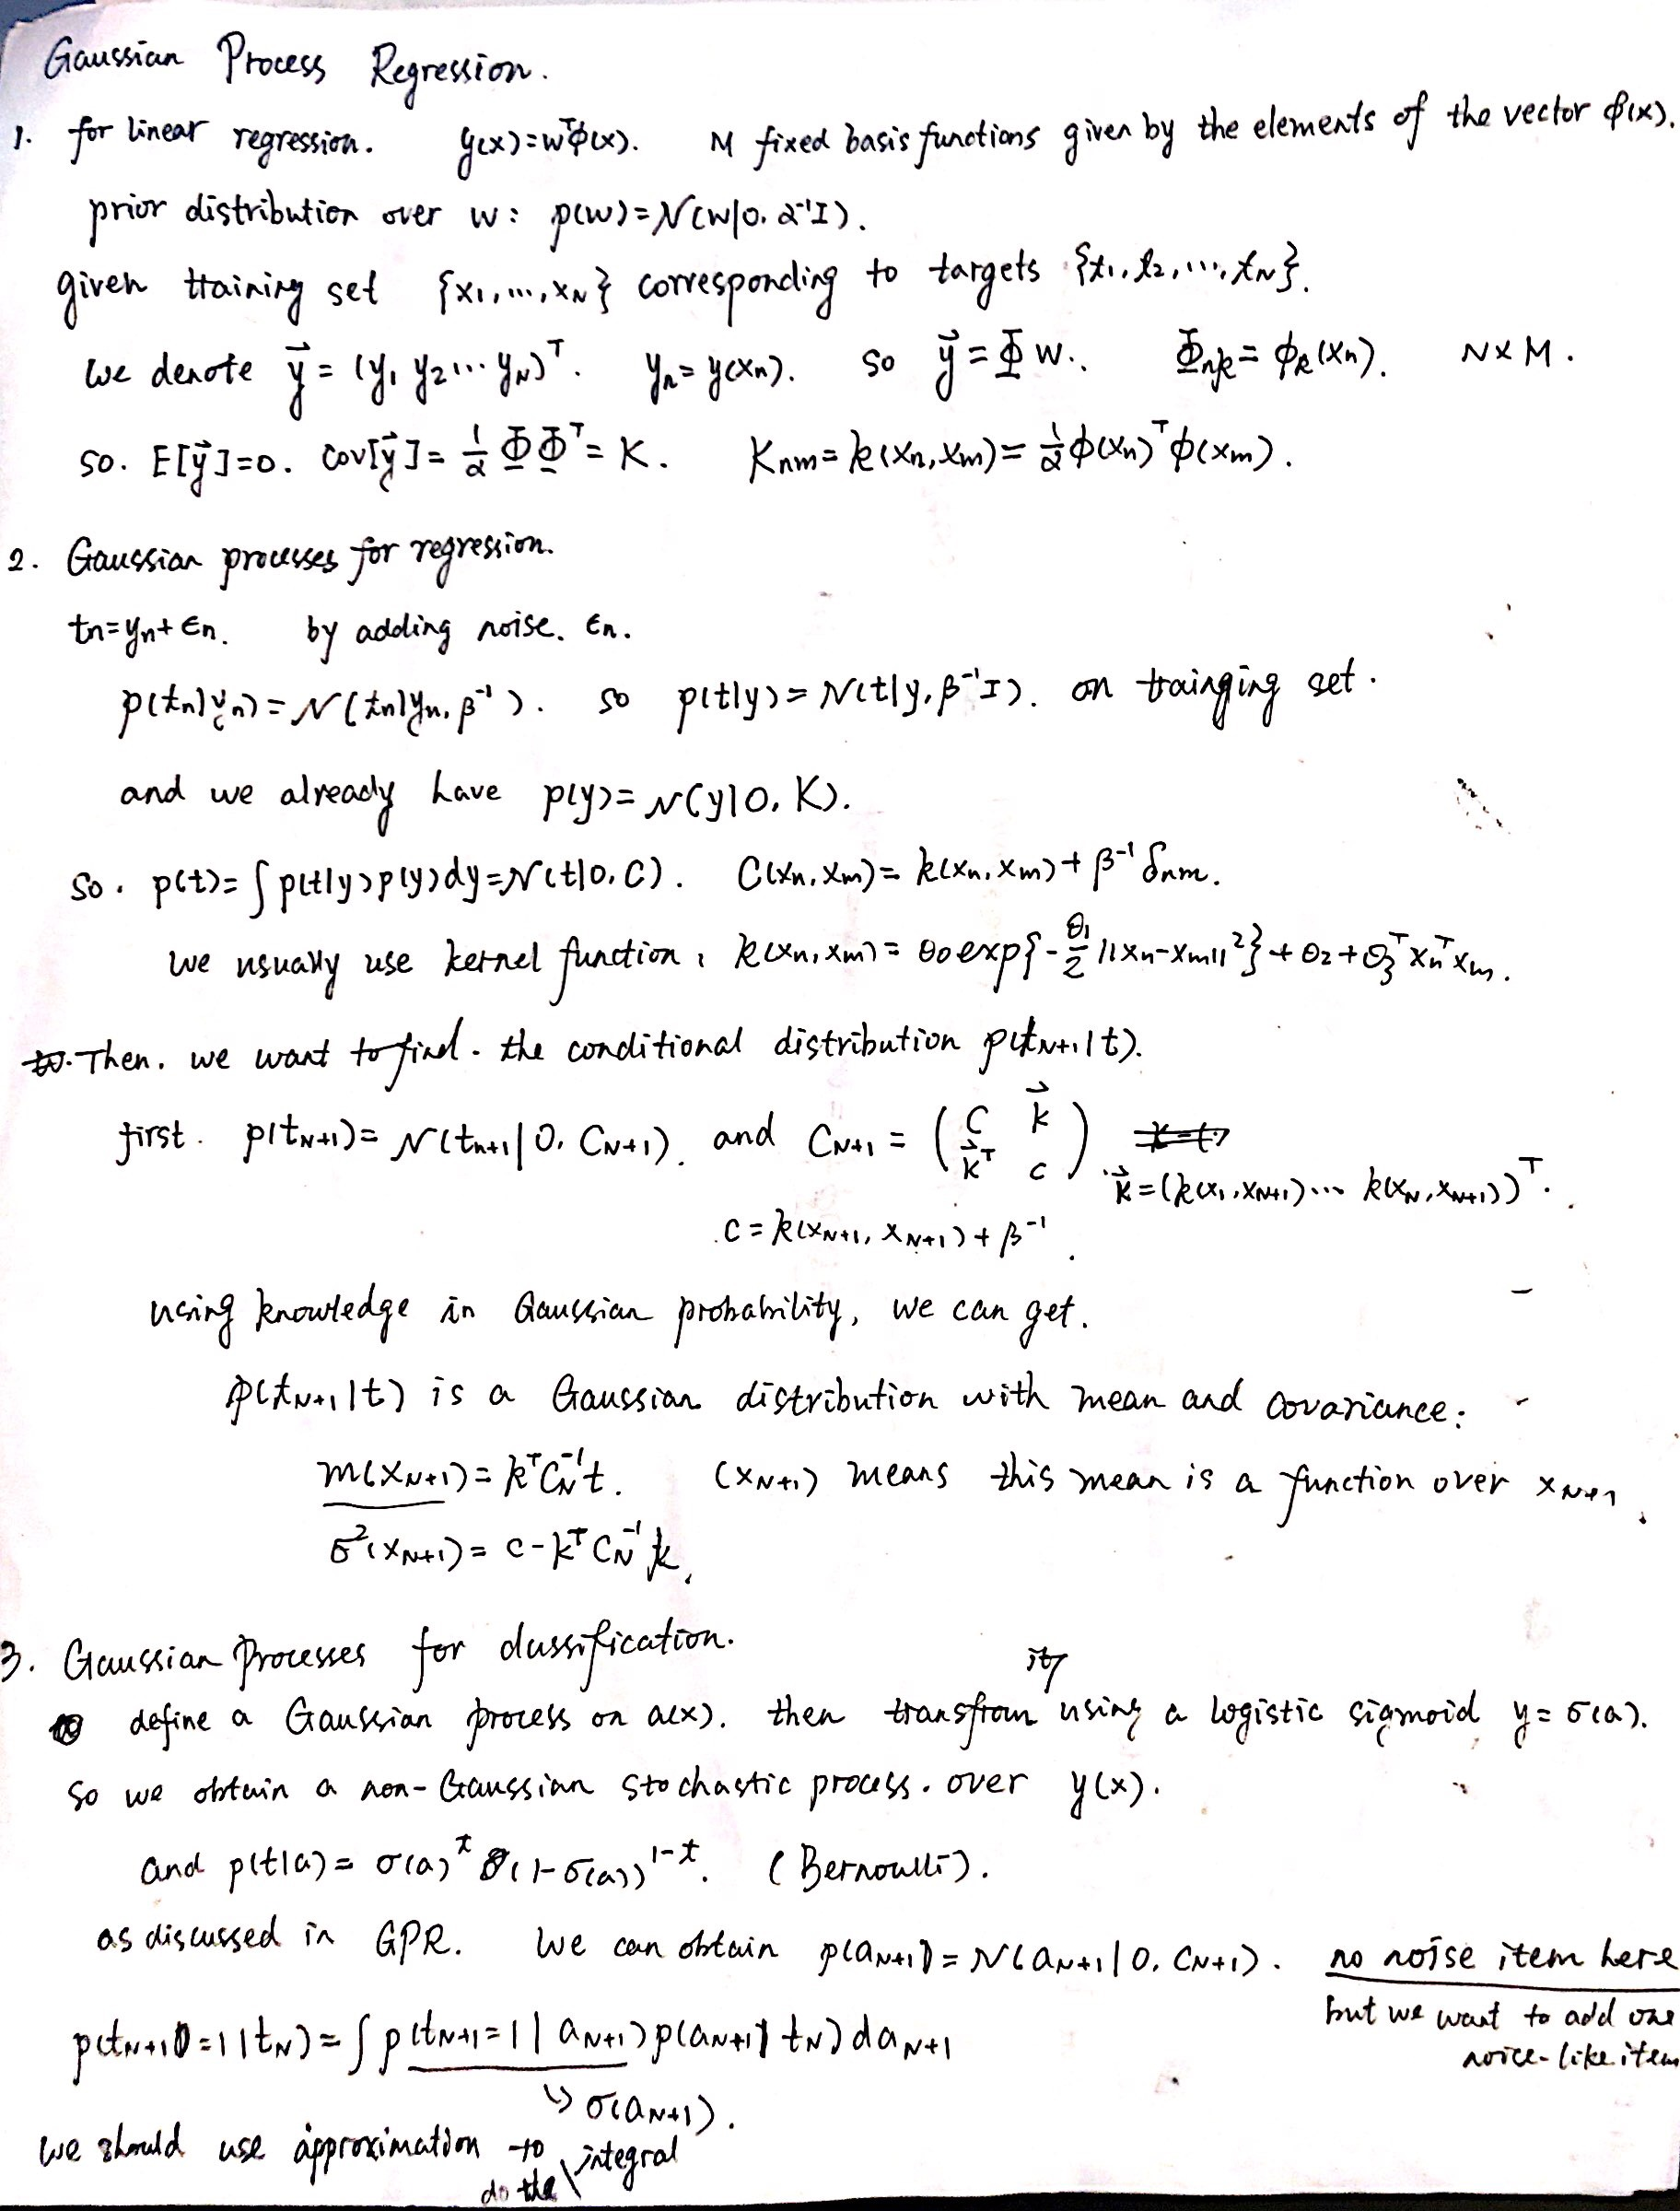
\includegraphics[width=\textwidth]{./imgs/GPR.jpg}
  \caption{Gaussian Process Regression}\label{fig3.5.1}
\end{figure}


\section{Sparse Kernel}
In this section we shall look at kernel-based algorithms that have sparse solutions, so that predictions for new inputs depend only on the kernel function evaluated at a subset of the training data points.\newline
\emph{SVM} is a decision machine and so does not provide posterior probabilities.
\textbf{property}: the  determination of the model parameters corresponds to a convex optimization problem, and so any local solution is also a global optimum.
\subsection{Maximum Margin Classifiers}
\emph{margin}: the smallest distance between the decision boudary and any of the samples.

In SVM: the decision boundary is chosen to be one for which the margin is maximized.

If the data set is not linearly seperable in the original space, we can project them into another feature space using basis functions $\phi()$  to make them seperable.

\uline{Don't quite understand the mathematical inference in this chapter.}  maybe I can try to discuss with other students in our reading group later.

More application of SVM will be focused on Multiclass SVMs, SVM for regression and overlapping classification.
\subsection{Relevance Vector Machines}
Limitation of SVM:
\begin{enumerate}
  \item the outputs of an SVM represent decisions rather than posterior probabilities.
  \item  the SVM was originally formulated for two classes, and the extension to $K > 2$ classes is problematic.
\end{enumerate}

And RVM is a Bayesian sparse kernel technique for regression and classification that shares many of the characteristics of the SVM whilst avoiding its principal limitations.

\subsubsection{For regression}
The most important difference between RVM and SVM is that we introduce a separate hyperparameter $\alpha_i$ for each of the weight $w_i$ instead of a single shared hyperparameters.
\subsubsection{For classification}
Because the prior distribution for classification problem is not the same as the regression problem, we can not integrate analytically  over the parameters.  So we should again use Laplace approximation technique to finish the inference.


\section{Graphical Models}
We shall find it highly advantageous to augment the analysis using diagrammatic representations of probability distributions, called \textit{probabilistic graphical models}. These offer several useful properties:
\begin{enumerate}
    \item They provide a simple way to visualize the structure of a probabilistic model and can be used to design and motivate new models.
    \item Insights into the properties of the model, including conditional independence properties, can be obtained by inspection of the graph.
    \item Complex computations, required to perform inference and learning in sophisticated models, can be expressed in terms of graphical manipulations, in which underlying mathematical expressions are carried along implicitly.
\end{enumerate}
\textit{nodes}: random variables. \textit{links}: probabilistic relationships between the variables.
\newline
\textit{Bayesan networks (directed graphical models)}, \textit{undirected graphical models}, \textit{factor graph}.

\subsection{Bayesian Networks}
Decomposition of a joint probability distribution:
\begin{equation}
    \tag{8.1} p(a, b, c) = p(c|a, b)p(b|a)p(a)
    \label{eq8.1}
\end{equation}
and the corresponding graphical model can be seen in figure\ref{GM1}.
\begin{figure}
\begin{minipage}{0.5\textwidth}
    \centering
    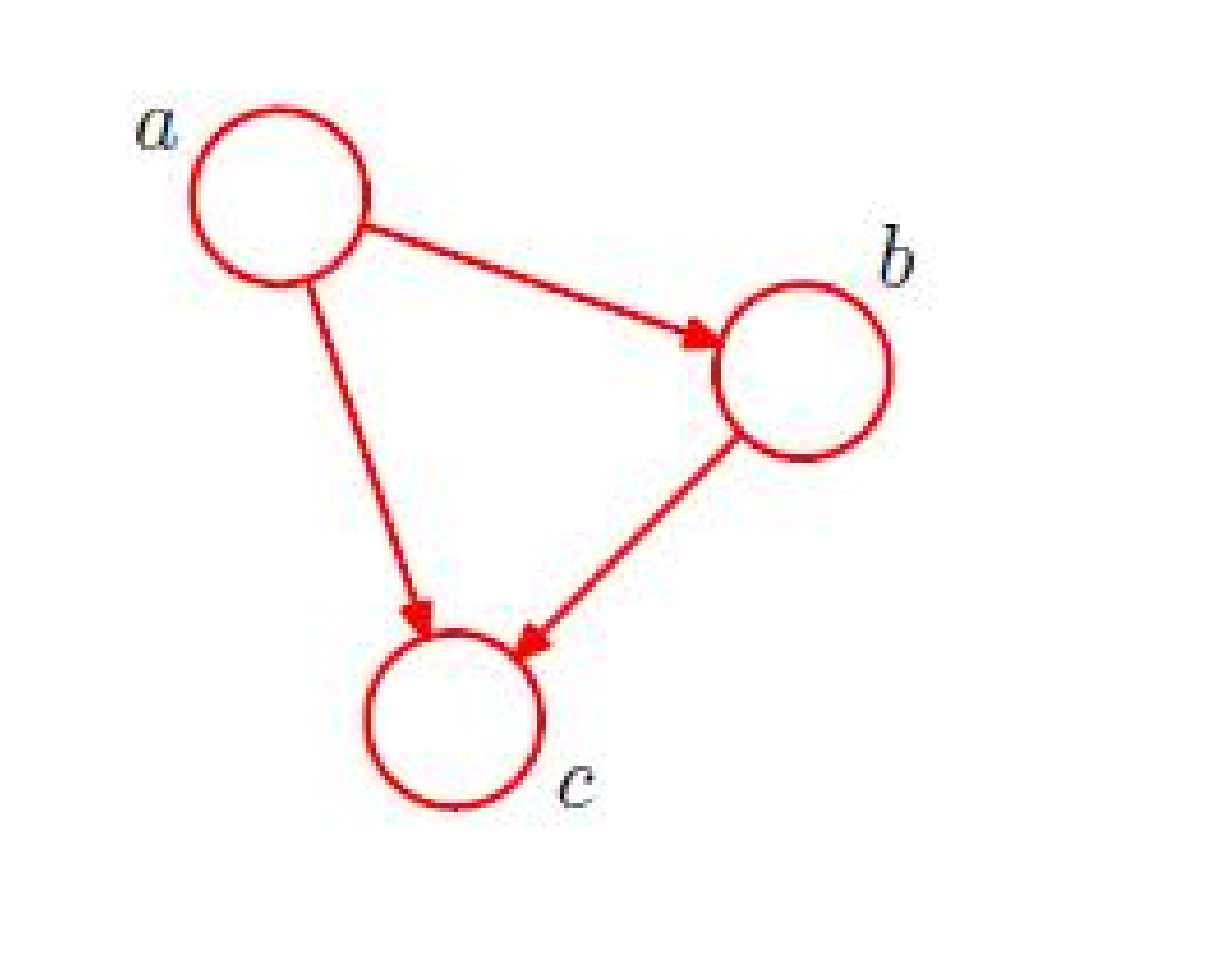
\includegraphics[width=0.5\linewidth]{./imgs/GM1.eps}
    \caption{}
    \label{GM1}
\end{minipage}
\begin{minipage}{0.5\textwidth}
    \centering
    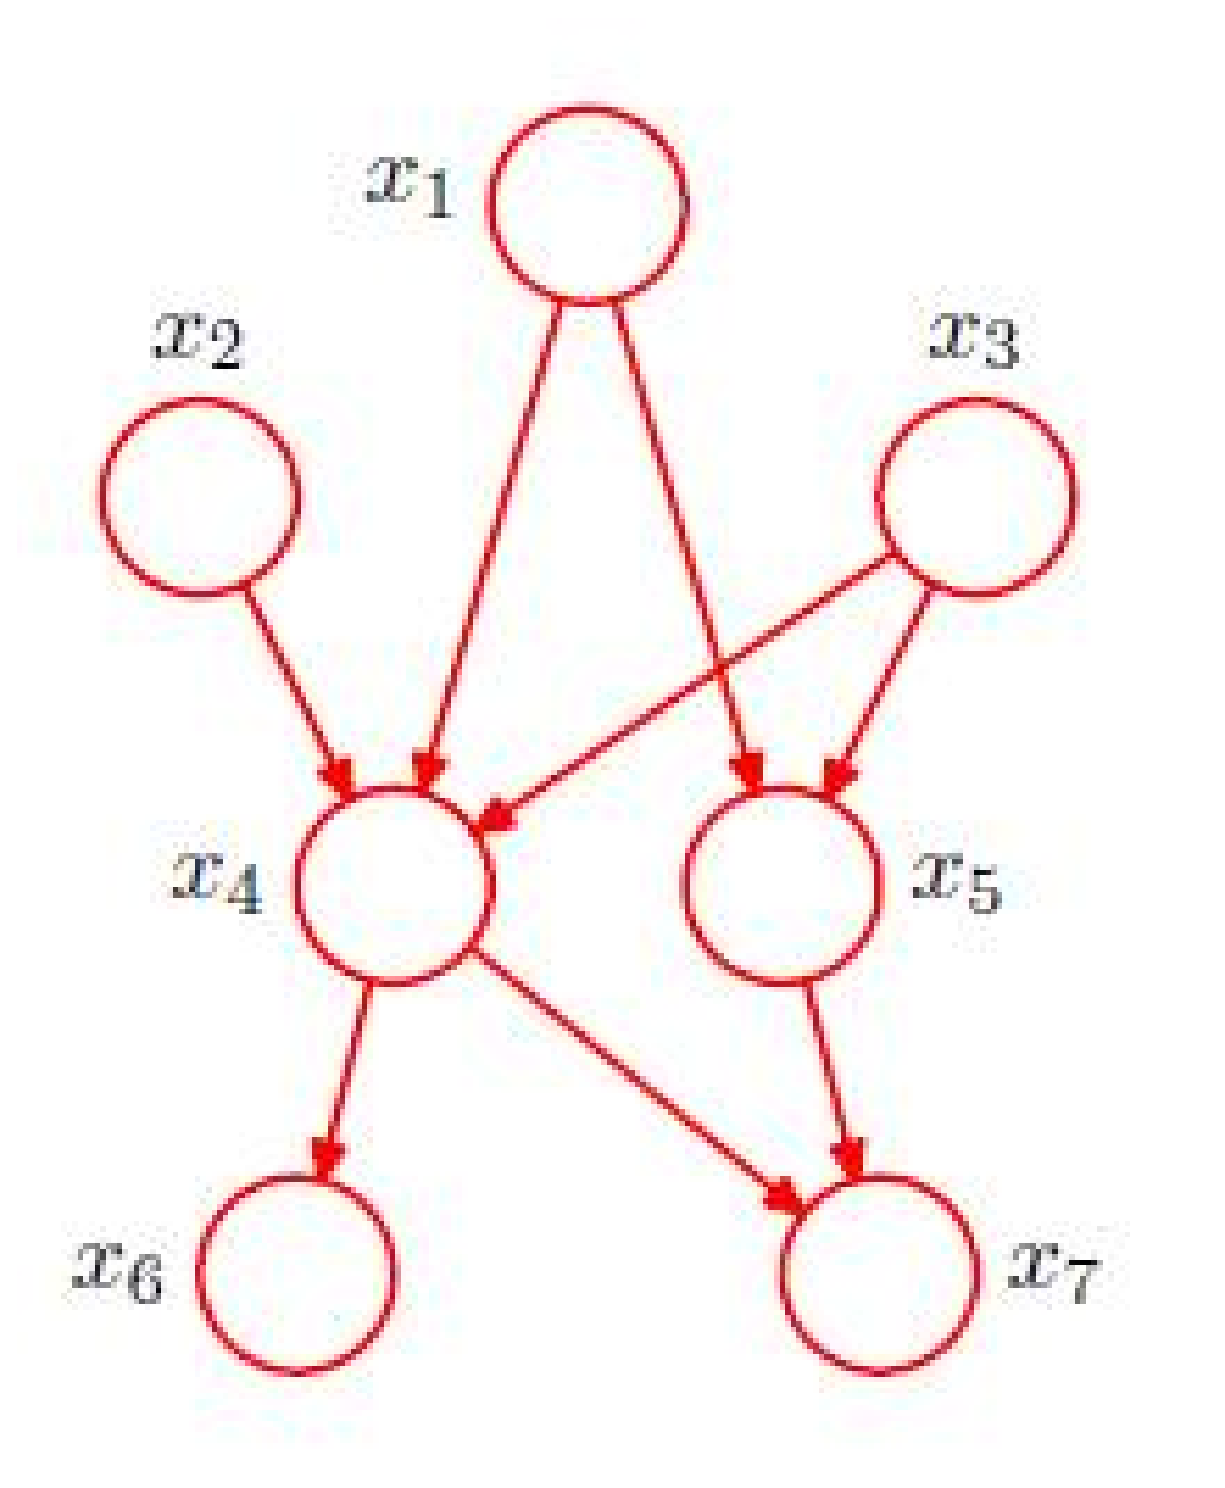
\includegraphics[width=0.5\linewidth]{./imgs/GM2.eps}
    \caption{}
    \label{GM2}
\end{minipage}
\end{figure}
\newline
\textbf{Rule}: for each conditional distribution we add directed links (arrows) to the graph from the nodes corresponding to the variables on which the distribution is conditioned.
\newline
we can extend the decomposition to $K$ variables:
\begin{equation}
    p(x_1,...,x_K) = p(x_K|x_1,...,x_{K-1})...p(x_2|x_1)p(x_1).
    \label{eq8.2}
\end{equation}
And the corresponding directed graph is called \textit{fully connected} because there is a link between every pair of nodes.
\newline
\textbf{Case} Given a directed graph as seen in \ref{GM2}, we can write the corresponding probability product:
\begin{equation}
    p(x_1)p(x_2)p(x_3)p(x_4|x_1,x_2,x_3)p(x_5|x_2,x_3)p(x_6|x_4)p(x_7|x_4,x_5)
    \label{8.3}
\end{equation}
\textbf{Rule}:
\begin{equation}
p(\textbf{x}) = \Pi_{k=1}^Kp(x_k|\mathrm{pa}_k)
\label{8.4}
\end{equation}
where $\mathrm{pa}_k$ denotes the set of parents of $x_k$, and $\textbf{x} = \{x_1,..,x_K\}$.
\newline
The directed graphs that we are considering are subject to an important restriction namely that there must be no \textit{directed cycles}, in other words there are no closed paths within the graph such that we can move from node to node along links following the direction of the arrows and end up back at the starting node. Such graphs are also called \textit{directed acyclic graphs}, or \textit{DAGs}. This is equivalent to the statement that there exists an ordering of the nodes such that there are no links that go from any node to any lower numbered node.
\subsubsection{Example: polynomial regression}
For more complex models, we shall adopt the convention that random variables will be denoted by open circles, and deterministic parameters will be denoted by smaller solid circles.
some concepts: \textit{observed variables, hidden variables, deterministic parameters}.
\subsubsection{Generative models}
\textit{sampling}: given a joint distribution, we want to draw a sample $\hat x_1, \hat x_2, ..., \hat x_K$ from it.
\textbf{ancestral sampling}
\newline
We start with the lowest-numbered node and draw a sample from the distribution $p(x_1)$, which we all $\hat x_1$. Then we work through each of the nodes in order, so that for node n we draw a sample from the conditional distribution p(xn|pan)
in which the parent variables have been set to their sampled values. Note that at each stage, these parent values will always be available because they correspond to lower-numbered
nodes that have already been sampled. The graphical model captures the \textit{causal} process by which the observed data was generated. For this reason, such models are often called \textit{generative} models. But the regression problem is not generative because there is no probability distribution associated with the input variable $x$, and it is not possible to generate synthetic data points from this model. But we can make it generative by introducing a suitable prior distribution $p(x)$, at the expense of a more complex model.
\subsubsection{Discrete variables}
\textit{parent-child pair in a directed graph. Two cases are particularly worthy of note, namely when the parent and child node each correspond to discrete variables and when they each correspond to Gaussian variables, because in these two cases the relationship can be extended hierarchically to construct arbitrarily complex directed acyclic graphs.}
\newline
\textbf{Case}:  discrete variable $\textbf{x}$ having $K$ possible states is given by
\begin{equation}\label{eq8.5}
  p(\bf{x}|\bf{mu}) =  \Pi_{k=1}^K\mu_k^{x_k}
\end{equation} governed by $\bf{\mu}$.
Suppose we have to discrete variables $\bf x_1, \bf x_2$, joint distribution can be written as
\begin{equation}\label{eq8.6}
  p(\bf x_1, \bf x_2|\bf{\mu})=\Pi_{k=1}^K\Pi_{k=1}^K\mu_{kl}^{x_{1k}x_{2l}}.
\end{equation}
$x_{1k}$ denotes the $k^{th}$ component of $\bf x_1$.
\newline
$K^2-1$ parameters. If we have $M$ variables, there is $K^M-1$ parameters, exponential with the num $M$.
\newline
Suppose $\bf x_1$ and $\bf x_2$ are independent. Each variable is then described by a separate multinomial distribution, and total number of parameters will be $2(K-1)$. If extend to $M$ variables, there will be $M(K-1)$ variables, linear growth.
\newline
\textbf{Generally case}: more links than independent variables but less links than a fully connected graph.
\newline
We can turn a graph over discrete variables into a Bayesian model by introducing Dirichlet priors for the parameters.
\newline
Another way of controlling the exponential growth in the number of parameters
in models of discrete variables is to use parameterized models for the conditional
distributions instead of complete tables of conditional probability values.
\subsubsection{Linear-Gaussian models}

\subsection{Conditional Independence}
If
\begin{equation}\label{eq8.7}
  p(a|b, c) = p(a|c),
\end{equation}
we say that $a$ is conditionally independent of $b$ given $c$, and we denote this by $$a\ci b|c .$$  And we will have
\begin{equation}\label{eq8.8}
  p(a,b|c) = p(a|c)p(b|c).
\end{equation}
\subsubsection{Examples}
Three examples related to conditional independence: \textit{tail-to-tail, head-to-tail, head-to-head}.
\subsubsection{D-separation}
We wish to ascertain whether a particular conditional
independence statement$$A\ci B |C$$is implied by a given directed acyclic graph.
\newline
i.i.d data points. Given $\mu$, we can say the data points $x_1,x_2,...,x_N$ are conditionally independent, but we can not say the data points are independent. because given $x_1$, the probability of $\mu$ will be affected and then $x_2$ will be affected.
\newline
\textbf{naive Bayes Model} Observation of $\bf{z}$ will block the path between $x_i$ and $x_j$ for $j\neq i$. So, if we are given a training set will, comprising inputs $\{x_1,...,x_N\}$ together with their labels, then we can fit the naive Bayes model to the training data using maximum likelihood assuming that the data are drawn independently from the model.
\newline
We can view a directed graph as a filter and all probability distribution $p(\bf x)$ that will be allowed through can make a set $\mathcal {DF}$.
\newline
\textbf{Markov blanket}.
\begin{equation}\label{eq8.9}
  p(\bf{x}_i|\bf{x}_{\{j\neq i\}}) = \frac{p(\bf x_1,...\bf x_D)}{\int p(\bf x_1,...,\bf x_D)\rm d\bf x_i}=\frac{\prod_k p(\bf x_k|\rm{pa}_k)}{\int \prod_k p(\bf x_k|\rm{pa}_k)\rm{d}\bf x_i}
\end{equation}
Some factors in $\prod_k p(\bf x_k|\rm{pa}_k)$ will disappear if they are not relative to $\bf x_i$.
\subsection{Markov Random Fields}
A \emph{Markov random field}, also known as a \emph{Markov network} or an \emph{undirected graphical model} , has a set of nodes each of which corresponds to a variable or group of variables, as well as a set of links each of which connects a pair of nodes. The links are undirected, that is they do not carry arrows.
\subsubsection{Conditional independence properties}
Properties in an undirected graph is much simpler than those in a directed graph because the nodes linked in a pair is symmetric, and there is no head-to-head situation. So if all paths that connect nodes in $A$ to nodes in $B$ pass through one or more nodes in the set $C$, then all such paths are 'blocked' and so the conditional independence property hold, aka. $$A\ci B|C$$.
\subsubsection{Factorization properties}
If two nodes are not linked directly, then we can obtain
\begin{equation}\label{eq8.10}
  p(x_i,x_j|\bf{x}_{\backslash\{i,j\}}) = p(x_i|\bf x_{\backslash\{i,j\}})p(x_j|\bf x_{\backslash\{i,j\}})
\end{equation}
\textbf{clique}:a subset of nodes in a graph such that there exists a link between all pairs of nodes in the subset. \newline
\textbf{maximal clique}:a clique such that it is not possible to include any
other nodes from the graph in the set without it ceasing to be a clique.\newline
Denote a clique by $C$ and the set of variables in that clique by $\bf x_C$. Then the joint distribution is written as a product of \emph{potential functions}
$\phi_C(\bf x_C)$ over maximal cliques of the graph
\begin{equation}\label{eq8.11}
  p(\bf x) = \frac{1}{Z}\prod_{C}\phi_C(\bf x_C).
\end{equation}
Here the quantity Z, sometimes called the partition function, is a normalization constant
and is given by
\begin{equation}\label{eq8.12}
  Z=\sum_{X}\prod_{C}\phi_C(\bf x_C)
\end{equation}
\emph{energy function} $E(\bf x_C)$
\begin{equation}\label{eq8.13}
  \phi_C(\bf x_C) = \exp\{-E(\bf x_C\}
\end{equation}
\subsubsection{Relation to directed graphs}
\begin{figure}
  \centering
  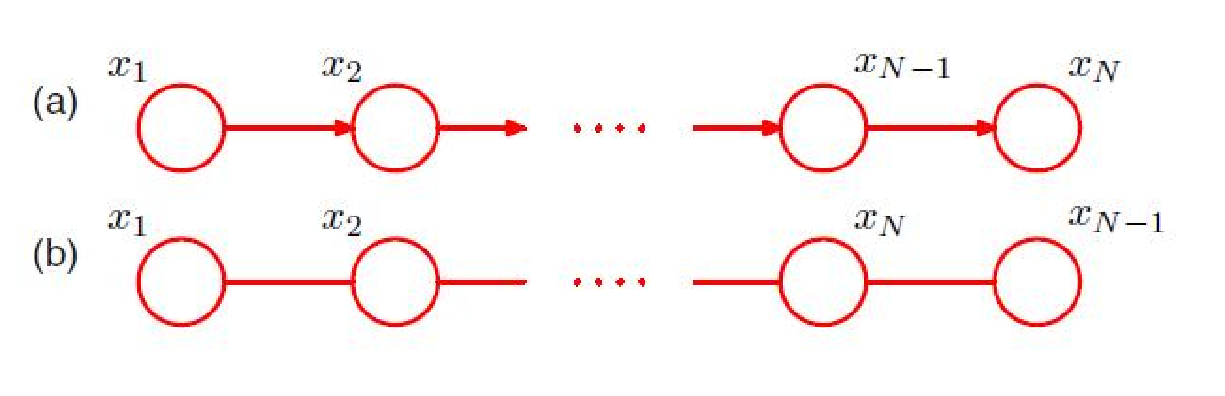
\includegraphics[width=\textwidth]{./imgs/GM3.eps}
  \caption{}\label{GM3}
\end{figure}
Given a directed graph as a chain shown in figure\ref{GM3}(a).
\begin{equation}\label{eq8.14}
  p(\bf x) =p(x_1)p(x_2|x_1)p(x_3|x_2)...p(x_N|x_{N-1})
\end{equation}
Also, for undirected graph shown in figure\ref{GM3}(b).
\begin{equation}\label{eq8.15}
  p(\bf x) = \frac{1}{Z}\psi_{1,2}(x_1,x_2)\psi_{2,3}(x_2,x_3)...\psi_{N-1,N}(x_{N-1},x_N).
\end{equation}
And we define
\begin{align}\label{eq8.15}
  \psi_{1,2}(x_1,x_2) = p(x_1)p(x_2|x_1) \\
  \psi_{2,3}(x_2,x_3)=p(x_3|x_2) \\
  \vdots \\
  \psi_{N-1,N}(x_{N-1},x_N) = p(x_N|x_{N-1})
\end{align}






\section{Continuous Latent Variables}
The simplest continuous latent variable model assumes Gaussian distributions
for both the latent and observed variables and makes use of a linear,Gaussian dependence of the observed variables on Ihe slate of the latent variables. This leads
to a probabilistic formulation of the well-known technique of principal component
analysis (PCA), as well as to a related model called factor analysis.
\subsection{Principal Component Analysis}

\section{FOR NEW}


\chapter{Algorithms}
\section{Nonparametric Methods}
In probability theory, we have  focussed on the use of probability distributions
having specific functional forms governed by a small number of parameters whose
values are to be determined from a data set.\textbf{This is called the parametric approach}.
\textbf{to density modelling}\newline
\textbf{histogram}
$$p_i = \frac{n_i}{N\Delta_i}=\frac{n_i}{N\Delta}$$
how to choose proper $\Delta$ is very important and sensitive
\subsection{Kernel density estimators}
Consider some small region $\mathcal R$ containing $\mathrm x$, the probability mass is given by
$$P=\int_{\mathcal R}p(\mathrm x)\mathrm {dx}$$
N observations drawn from $p(\mathrm x)$ \newline
Total number $K$ of points that lie inside $\mathcal R$ will be distributed according to the binomial distribution.
$$\mathrm {Bin}(K|N,P) =$$
so mean faction in the region will be $\mathrm E[K/N] = P$, and $\mathrm {var}[K/N] = P(1-P)/N$.\newline
$P=p(\mathrm x)V$ if $\mathcal R$ is small enough, so $p(\mathrm x) = \frac{K}{NV}$\newline
\textbf{based on two contradictory assumptions}: region is sufficiently small that the density is approximately constant over the region and yet sufficiently large that the number $K$ of points falling inside the region is sufficient for the binomial distribution to be sharply peaked.\newline
If we fix $V$ and determine $K$ from the data,  giving rise to the kernel approach.
$k(\mathrm u) =1$ if $|u_i|\leq 1/2, i=1, 2, \dots, D, $ else $0$ .\newline
This represents a unit cube centred on the origin. The function $k(\mathrm u)$ is an example of a \emph{kernel function}\newline
So $$K = \sum_{n=1}^Nk(\frac{\mathrm x-\mathrm x_n}{h}), p(\mathrm x) = \frac1N\sum_{n=1}^N\frac1{h^D}k(\frac{\mathrm x-\mathrm x_n}{h})$$
and common choice for a kernel is Gaussian, which give rise to the following kernel density model:
$$p(\mathrm x) = \frac1N\sum_{n=1}^N\frac{1}{(2\pi h^2)^{1/2}}\exp\{-\frac{||\mathrm x-\mathrm x_n||^2}{2h^2}\}$$
also a trade-off between sensitivity to noise at small $h$ and over-smoothing at large $h$\newline
computational cost.
\subsection{Nearest-neighbour methods}
idea: allow the radius of the sphere to grow until it contains precisely $K$ data points, then the volume of the sphere is set to $V$.\newline
K-nearest-neighbour technique for density estimation can be extended to classification.
$N_k$ points in class $\mathcal C_k$, $\sum_kN_k=N$
\newline
If we want to classify a new point $\mathrm x$, we draw a sphere centred on $\mathrm x$ containing precisely $K$ points. Suppose this sphere contains $K_k$ points from $\mathcal C_k$. Then
$$p(\mathrm x|\mathcal C_k) = \frac{K_k}{N_kV} , p(\mathrm x) = \frac{K}{NV}, p(\mathcal C_k) = \frac{N_k}{N}$$
so $p(\mathcal C_k|\mathrm x) = \frac{K_k}{K}$
\section{Inference Algorithms in Graphical Models}
\subsection{Inference on a chain}
Consider the graph shown in figure\ref{GM3}. The joint distribution for this graph takes the form
\begin{equation}\label{eq8.16}
  p(\bf x) = \frac{1}{Z}\psi_{1,2}(x_1,x_2)\psi_{2,3}(x_2,x_3)...\psi_{N-1,N}(x_{N-1},x_N).
\end{equation}
If we want to get marginal distribution $p(x_n)$ for a specific node, we should sum the joint distribution over all variables except $x_n$, so that
\begin{equation}\label{eq8.17}
  p(x_n) = \sum_{x_1}...\sum_{x_{n-1}}\sum_{x_{n+1}}...\sum_{x_N}p(\bf x)
\end{equation}
But this way will cost so much computational resources, so we want to find another simpler way:
\begin{align}\label{eq8.18}
  p(x_n) =  & \frac{1}{Z}[\sum_{x_{n-1}}\psi_{n-1,n}(x_{n-1},x_n)\dots[\sum_{x_2}\psi_{2,3}(x_2,x_3)[\sum_{x_1}\psi_{1,2}(x_1,x_2)]]\dots] \\
   & [\sum_{x_{n+1}}\psi_{n,n+1}(x_n,x_{n+1})\dots[\sum_{x_N}]\psi_{N-1,N}(x_{N-1},x_{N})]\dots]  \\
   = & \frac{1}{Z}\mu_{\alpha}(x_n)\mu_{\beta}(x_n)
\end{align}
As shown in figure\ref{GM4}, we can see message passed in the chain and we can compute $\mu_{\alpha}(x_i)$ and $\mu_{\beta}(x_i)$ recursively for any $i=1, 2, \dots, N$.
\begin{equation}\label{eq8.19}
  \mu_{\alpha}(x_n) = \sum_{x_{n-1}}\psi_{n-1,n}(x_{n-1},x_n)\mu_{\alpha}(x_{n-1}).
\end{equation}
and
\begin{equation}\label{eq8.20}
  \mu_{\alpha}(x_2) = \sum_{x_1}\psi_{1,2}(x_1,x_2).
\end{equation}
Similar for $\mu_{\beta}(x_n)$
\begin{figure}[bth]
  \centering
  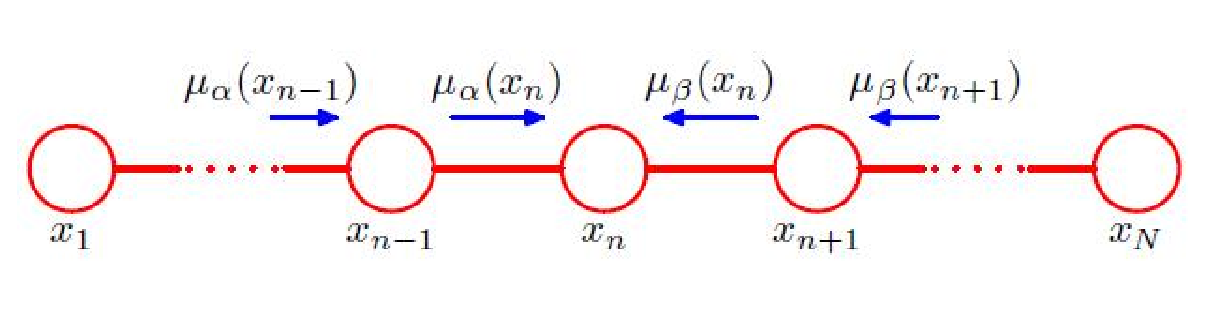
\includegraphics[width=\textwidth]{./imgs/GM4.eps}
  \caption{}\label{GM4}
\end{figure}
\subsection{Inference on a tree: sum-product algorithm}
Tree do not have loops.
\subsubsection{factor graphs}
In a factor graph, there is a node (depicted as usual by \textbf{a circle}) for every variable
in the distribution, as was the case for directed and undirected graphs. There are also
additional nodes (depicted by \textbf{small squares}) for each factor fs(xs) in the joint distribution.\newline
For example,
\begin{equation}\label{eq8.21}
  p(\bf{x}) = f_a(x_1,x_2)f_b(x_1,x_2)f_c(x_2,x_3)f_d(x_3)
\end{equation}
can be expressed by the factor graph shown in figure\ref{GM5}
\begin{figure}
  \centering
  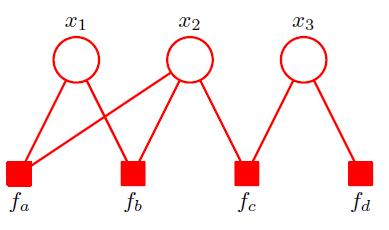
\includegraphics[width=0.5\textwidth]{./imgs/GM5.jpg}
  \caption{Example of a factor graph}\label{GM5}
\end{figure}
Factor graphs are said to be bipartite because they consist of two distinct kinds
of nodes, and all links go between nodes of opposite type.
\subsubsection{sum-product algorithm}
We shall now make use of the factor graph framework to derive a powerful class
of efficient, exact inference algorithms that are applicable to tree-structured graphs.
Here we shall focus on the problem of evaluating local marginals over nodes or
subsets of nodes, which will lead us to the sum-product algorithm.\newline
Our goal is to exploit the structure of
the graph to achieve two things: (i) to obtain an efficient, exact inference algorithm
for finding marginals; (ii) in situations where several marginals are required to allow
computations to be shared efficiently.
\textbf{finding the marginal $p(x)$ for a particular variable node $x$}\newline
$$p(\bf x) = \prod_{s\in ne(x)}F_s(x,X_s)   $$
$$p(x) = \prod_{s\in ne(x)}[\sum_{X_s}F_s(x,X_s)] = \prod_{s\in ne(x)}\mu_{f_s\rightarrow x}(x) $$
$$F_s(x,X_s) =  f_s(x,x_1,...x_M)G_1(x,X_{s1})...G_M(x,X_{sM})$$
$$\mu_{x_m\rightarrow f_s}(x_m) \equiv \sum_{X_{sm}}G_m(x_m,X_{sm})$$
We have therefore introduced two distinct kinds of message, those that go from factor
nodes to variable nodes denoted $\mu_{f\rightarrow x}(x)$, and those that go from variable nodes to
factor nodes denoted $\mu_{x\rightarrow f}(x).$
\textbf{Illustration: example}
\textbf{max-sum algorithm}
Two other common tasks are to find a setting of the variables that has the largest probability
and to find the value of that probability. We therefore seek an efficient algorithm for finding the value of x that maximizes
the joint distribution p(x) and that will allow us to obtain the value of the
joint distribution at its maximum.
\subsection{Exact inference in a general graph}
Goal: deal with graphs having loops.\newline
\textbf{Loopy belief progpagation}
One simple approach to approximate inference in graphs with
loops, which builds directly on the previous discussion of exact inference in trees.
The idea is simply to apply the sum-product algorithm even though there is no guarantee
that it will yield good results. For some graphs, the algorithm will converge, whereas for others it will not. \newline
We will say that a (variable or factor) node a has a message pending on its link to a node b if node a has received any
message on any of its other links since the last time it send a message to b.

\section{Mixture Models and EM}
This section is mainly about chap.9 in \textbf{PRML}.\newline
We can use mixture models to cluster data, as well as build more complex probability distributions. Therefore we begin our discussion of mixture distributions by considering the problem of finding clusters in a set of data points. Then we introduce the latent variable view of mixture distributions in which the discrete variables can be interpreted as defining assignments of data points to specific component of the mixture. Finally we discuss EM in some generality.
\subsection{K-means Clustering}
Suppose we have a data set $\{\mrm x_1,\cdots, \mrm x_N\}$ consisting of $N$ observations of a random $D-$dimensional Euclidean variable $\mrm x$. Our goal is to partition the data set into some number $K$ of clusters.  Firstly we consider a fixed value of $K$. We can formalize this notion by first introducing a set of $D-$dimensional vectors $\mu_k$, where $k=1,\cdots,K$, in which $\mu_k$ is a prototype associated with the $k^{th}$ cluster. For each data point $\mrm x_n$, we introduce a corresponding set of binary indicator variables $r_{nk} \in \{0,1\}$, describing which cluster $\mrm x_n$ is assigned to. We can then define an objective function
\begin{equation}
J = \sum_{n=1}^{N}\sum_{k=1}^{K}r_{nk}\|\mrm x_n-\mu_k\|^2.
\end{equation}
Firstly we choose some initial values for the $\mu_k$. Then in the first phase we minimize $J$ with respect to the $r_{nk}$, keeping the $\mu_k$ fixed. In the second phase we minimize $J$ with respect to the $\mu_k$, keeping $r_{nk}$ fixed. This two-stage optimization is then repeated until convergence. And we obtain
\begin{gather}\label{}
  r_{nk}=\{\begin{matrix}
                 1 & \mrm{if }k=\mrm{arg min_j}\|\mrm x_n-\mu_j\|^2 \\
                 0 & \mrm{otherwise}.
               \end{matrix} \\
  \mu_k = \frac{\sum_nr_{nk}\mrm x_n}{\sum_nr_{nk}}
\end{gather}
A direct implementation of the $K-$means algorithm as discussed here cna be slow because in each E step it is necessary to compute the Euclidean distance between every prototype vector and every data point. Various schemes have been proposed for speeding up this algorithm.

\subsection{Mixtures of Gaussians}
Recall from previous chapter the Gaussian mixture distribution can be written as linear superposition of Gaussians  in the form
\begin{equation}\label{}
  p(\mbf x) = \sum_{k=1}^{K}\pi_k\normD(\mbf x|\mu_k,\Sigma_k).
\end{equation}
Then we can introduce a $K-$dimensional binary random variable $\mbf z$ having a 1-of-$K$ representation in which a particular element $z_k$ is equal to 1 and all other elements are equal to 0. So $z_k \in \{0,1\}$, $\sum_{k}z_k=1$, and $p(z_k=1)=\pi_k$. So
\begin{equation}\label{}
  p(\mrm z) = \prod_{k=1}^{K}\pi_k^{z_k}.
\end{equation}
Similarly, the conditional distribution of $\mrm x$ given a particular value for $\mrm z$ is a Gaussian
\begin{equation}\label{}
  p(\mrm x|z_k=1) = \normD(\mrm x|\mu_k, \Sigma_k).
\end{equation}
So the marginal distribution of $\mrm x$ is then obtained:
\begin{equation}\label{}
  p(\mrm x) = \sum_{\mrm z}p(\mrm z)p(\mrm x|\mrm z) = \sum_{k=1}^{K}\pi_k\normD(\mrm x|\mu_k,\Sigma_k)
\end{equation}
And we can gain the conditional probability of $\mrm z$ given $\mrm x$ using Bayes' theorem
\begin{equation}\label{eq3.3.0}
  \gamma(z_k) \equiv p(z_k=1|\mrm x)=\frac{p(z_k=1)p(\mrm x|z_k=1)}{\sum_{j=1}^{K}p(z_j=1)p(\mrm x|z_j=1)} =  \frac{\pi_k\normD(\mrm x|\mu_k, \Sigma_k)}{\sum_{j=1}^{K}\pi_j\normD(\mrm x|\mu_j,\Sigma_j)}.
\end{equation}
\subsubsection*{Maximum likelihood}
Suppose we have a data set of observations $\{\mrm x_1, \cdots, \mrm x_N\}$, and we wish to model this data using a mixture of Gaussians. Denote this data set as an $N\times D$ matrix $\mrm X$ in which the $n^{th}$ row is given by $\mrm x_n^T$, latent variables as an $N\times K$ matrix $\mrm Z$ with rows $\mrm z_n^T$. Assume i.i.d observations, we can obtain
\begin{equation}\label{}
  \ln p(\mrm X|\pi, \mu, \Sigma) = \sum_{n=1}^{N}\ln\{\sum_{k=1}^{K}\pi_k\normD(\mrm x_n|\mu_k, \Sigma_k)\}.
\end{equation}
Here, we may encounter a significant problem about singularity.
\subsubsection*{EM for Gaussian mixtures}
Setting the derivatives of $\ln p(\mrm X|\pi,\mu,\Sigma)$ with respect to the means $\mu_k$ of the Gaussian components to zero, we obtain
\begin{equation}\label{}
  0=-\sum_{n=1}^{N}\frac{\pi_k\normD (\mrm x_n|\mu_k,\Sigma_k)}{\sum_j\pi_j\normD(\mrm x_n|\mu_j,\Sigma_j)}\Sigma_k(\mrm x_n-\mu_k).
\end{equation}
We assume $\Sigma_k$ to be nonsingular so
\begin{equation}\label{eq3.3.1}
  \mu_k=\frac{1}{N_k}\sum_{n=1}^{N}\gamma(z_{nk})\mrm x_n
\end{equation}
where we have defined
\begin{equation}\label{}
  N_k \equiv \sum_{n=1}^{N}\gamma(z_{nk})
\end{equation}
We see that the mean $\mu_k$ for the $k^{th}$ Gaussian
component is obtained by taking a weighted mean of all of the points in the data set,
in which the weighting factor for data point $\mrm x_n$ is given by the posterior probability
$\gamma(z_{nk})$ that component $k$ was responsible for generating $\mrm x_n$.

If we set the derivative of $\ln p(\mrm X|\pi,\mu,\Sigma)$ with respect to $\Sigma_k$ to zero , we obtain
\begin{equation}\label{eq3.3.2}
  \Sigma_k=\frac{1}{N_k}\sum_{n=1}^{N}\gamma(z_{nk})(\mrm x_n-\mu_k)(\mrm x_n-\mu_k)^T.
\end{equation}

Finally we maximize $\ln p(\mrm X|\pi,\mu,\Sigma)$ with respect to $\pi_k$ using a Lagrange multiplier and we obtain
\begin{equation}\label{eq3.3.3}
  \pi_k=\frac{N_k}{N}
\end{equation}
We must emphasize that these results \ref{eq3.3.1}, \ref{eq3.3.2}, \ref{eq3.3.3} do not constitute a close-form solution for the parameters of the mixture model because $\gamma(z_{nk})$ depend on those parameters. But we can use the EM algorithm in a simple iteration:
\begin{enumerate}
  \item Initialize the means $\mu_k$, covariances $\Sigma_k$ and mixing coefficients $\pi_k$, and evaluate the initial value of the log likelihood.
  \item \textbf{E step.} Evaluate the responsibilities using the current parameter values using \ref{eq3.3.0}
  \item \textbf{M step.} Re-estimate the parameters using the current responsibilities using \ref{eq3.3.1}, \ref{eq3.3.2},\ref{3.3.3}.
  \item Evaluate the log likelihood
  \begin{equation}\label{}
    \ln p(\mrm X|\mu,\Sigma,\pi)=\sum_{n=1}^{N}\ln \{\sum_{k=1}^{K}\pi_k\normD(\mrm x_n|\mu_k,\Sigma_k)\}
  \end{equation}
\end{enumerate}

\subsection{An Alternative View of EM}
In this section, we present a complementary view of the EM algorithm that recognizes the key role played by latent variables.

Denote:
\begin{itemize}
  \item $\mrm X$: all observed data, $n^{th}$ row represents $\mrm x_n^T$.
  \item $\mrm Z$: all latent variables, $n^{th}$ row represents $\mrm z_n^T$.
  \item $\theta$: all model parameters.
\end{itemize}
So the log likelihood function is given by
\begin{equation}\label{}
  \ln p(\mrm X|\theta) = \ln\{\sum_{\mrm z}p(\mrm X,\mrm Z|\theta)\}.
\end{equation}
In practice, we are given only incomplete data set $\mrm X$ rather than complete $\{\mrm{X,Z}\}$, so our state of knowledge of the latent variables in $\mrm Z$ is given only by the posterior distribution $p(\mrm Z|\mrm X,\theta)$.

So the general EM algorithm is summarized below. Given a joint distribution $p(\mrm X,\mrm Z|\theta)$ over observed variables $\mrm X$ and latent variables $\mrm Z$, governed by parameters $\theta$, the goal is to maximize the likelihood function $p(\mrm X|\theta)$ with respect to $\theta$.
\begin{enumerate}
  \item Choose an initial setting for the parameters $\theta^{\mrm{old}}$.
  \item \textbf{E step} Evaluate $p(\mrm Z|\mrm X, \theta^{\mrm{old}})$.
  \item \textbf{M step} Evaluate $\theta^{\mrm{new}}$ given by 
  \begin{equation}\label{}
    \theta^{\mrm{new}} = \mrm{argmax}_\theta \mathcal Q(\theta,\theta^{\mrm{old}})
  \end{equation} 
  where 
  \begin{equation}\label{}
    \mathcal Q(\theta,\theta^{\mrm{old}}) = \sum_\mrm{z} p(\mrm Z|\mrm X,\theta^{{\mrm{old}}})\ln p(\mrm X,\mrm Z|\theta).
  \end{equation}
  \item Check for convergence of either the log likelihood or the parameter values. If the convergence criterion is not satisfied, then let
  \begin{equation}\label{}
    \theta^{\mrm{old}} \leftarrow \theta^{\mrm{new}} 
  \end{equation}
  and return to step 2.
\end{enumerate}

\subsubsection*{Gaussian mixtures revisited}
Consider the problem of maximizing the likelihood for the complete data set $\{\mrm X,\mrm Z\}$
\begin{equation}\label{}
  p(\mrm{X,Z}|\mu,\Sigma,\pi) = \prod_{n=1}^{N}\prod_{k=1}^{K}\pi_k^{z_{nk}}\normD(\mrm x_n|\mu_k,\Sigma_k)^{z_{nk}}
\end{equation}
where $z_{nk}$ denotes the $k^{th}$ component of $\mrm z_n$. Taking logarithm and 
\begin{equation}\label{}
  \ln p(\mrm{X,Z}|\mu,\Sigma,\pi) = \sum_{n=1}^{N}\sum_{k=1}^{K}z_{nk}\{\ln \pi_k+\ln\normD(\mrm x_n|\mu_k,\Sigma_k)\}.
\end{equation}
Consider first the maximization with respect to the means and covariances. 
\begin{equation}\label{}
  \pi_k = \frac1N\sum_{n=1}^{N}z_{nk}
\end{equation}
so that the mixing coefficients are equal to the fractions of data points.
\begin{equation}\label{}
  \mrm E[z_{nk}] = \gamma(z_{nk}
\end{equation}
\begin{equation}\label{}
  \mrm E_{\mrm z}[\ln p(\mrm X,\mrm Z|\mu,\Sigma,\pi)] =\sum_{n=1}^{N}\sum_{k=1}^{K}\gamma(z_{nk})\{\ln \pi_k+\ln \normD(\mrm x_n|\mu_k,\Sigma_k)\}.
\end{equation}

\subsubsection*{Relation to K-means}

\subsection{The EM Algorithm in General}
EM algorithm is a general technique for finding maximum likelihood solutions for probabilistic models having latent variables. Here we give a very general treatment of the EM algorithm. 

Consider, observed variables $\mrm X$, latent variables $\mrm Z$ and parameters $\theta$. Our goal is to maximize the likelihood function given by 
\begin{equation}\label{}
  p(\mrm X|\theta)=\sum_{\mrm z}p(\mrm X,\mrm Z|\theta).
\end{equation}
Suppose that direct optimization of $p(\mrm X|\theta)$ is difficult, but that optimization of the complete-data likelihood function $p(\mrm X,\mrm Z|\theta)$ is easier. Next we introduce a distribution $q(\mrm Z)$ defined over the latent variables, and 
\begin{equation}\label{}
  \ln p(\mrm X|\theta) = \mathcal L(q,\theta)+\mrm{KL}(q\|p)
\end{equation} 
where 
\begin{gather}\label{}
  \mathcal L(q,\theta) = \sum_{\mrm z}q(\mrm Z)\ln\{\frac{p(\mrm X,\mrm Z|\theta)}{q(\mrm Z)}\} \\
  \mrm {KL}(q\|p)=-\sum_{\mrm z}q(\mrm Z)\ln\{\frac{p(\mrm Z|\mrm X,\theta)}{q(\mrm Z)}\}.
\end{gather}
 Suppose the current value of the parameter vector is $\theta^{old}$. In the E step, the lower bound $\mathcal L(q,\theta^{old})$ is maximized with respect to $q(\mrm Z)$ while holding $\theta^{old}$ fixed. 
 
 In the subsequent M step, the distribution $q(\mrm Z)$ is held fixed and the lower bound $\mathcal L(q, \theta)$ is maximized with respect to $\theta$ to give some new value $\theta^{new}$. 
 
\end{document} 